\documentclass[conference]{IEEEtran}
\usepackage{amsmath,amssymb}
\usepackage{booktabs}
\usepackage{graphicx}
\usepackage{url}
\usepackage{xcolor}
\usepackage{array}
\usepackage{multirow}
\usepackage{hyperref}
\hypersetup{colorlinks=true,linkcolor=black,citecolor=black,urlcolor=blue}
\graphicspath{{../backend/app/assets/experiments/}{../results/task4/results/evaluation_results/}{../graphs/}}

\title{A Containerized Generative AI Application for\\
Universal Restoration, Hard-Routed Restoration, and\\
Style-Conditioned Face-to-Sketch Generation}

\author{\IEEEauthorblockN{Akif Jawad}\IEEEauthorblockA{Generative AI Assignment 1\\FAST Islamabad\\\url{https://github.com/AKIF-jk/Generative_AI}}}

\begin{document}
\maketitle

\begin{abstract}
\normalfont
This paper presents a reproducible generative-AI application containing three completed workspaces: universal multi-corruption image restoration, corruption classification with hard-routed specialist autoencoders, and style-conditioned face-to-sketch generation. The restoration experiments use the Oxford-IIIT Pet dataset with runtime corruption synthesis and deterministic validation/test manifests. The sketch system uses paired FS2K photographs and sketches, a conditional U-Net generator, and a PatchGAN discriminator. All inference models are exported to ONNX and served through FastAPI; a React/Vite frontend provides upload, corruption, routing, style, visualization, metric, and download controls. The universal restoration model obtains mean test L1 $=0.02710$ and SSIM $=0.89721$. The hard-routing classifier obtains accuracy $=0.99210$ and macro-F1 $=0.98725$; predicted routing obtains L1 $=0.05574$ and SSIM $=0.76287$. The face-to-sketch generator obtains overall L1 $=0.22262$ and SSIM $=0.46273$ on 1,045 evaluation examples. Task 3, the soft mixture-of-experts system, is explicitly outside the scope of this submission and is not claimed as complete.
\end{abstract}

\begin{IEEEkeywords}
image restoration, autoencoder, hard routing, conditional GAN, U-Net, PatchGAN, ONNX, FastAPI, React
\end{IEEEkeywords}

\section{Introduction}
Image restoration and paired image-to-image translation are useful testbeds for understanding how data pipelines, inductive biases, losses, hyperparameter optimization, and deployment decisions interact. This assignment requires four related generative systems and a browser application through which an evaluator can upload unseen images, inspect intermediate information, and download outputs. The work reported here focuses on the completed Tasks 1, 2, and 4. Task 3 was intentionally not undertaken; therefore, the paper reports the exclusion as a limitation rather than presenting unsupported results.

The project addresses three questions. First, can one compressed convolutional autoencoder restore several corruption families without being told which corruption occurred? Second, does a classifier followed by independently trained specialists improve interpretability and specialization? Third, can a conditional adversarial model learn style-dependent mappings from facial photographs to sketches while retaining paired-image fidelity?

The main contributions of the completed work are: (i) an explicit runtime corruption pipeline with protected deterministic manifests; (ii) an ONNX-exported universal restoration model and a hard-routing ensemble with operational and oracle evaluation; (iii) a style-conditioned U-Net/PatchGAN implementation with a learned embedding fused into both networks; (iv) a containerized FastAPI--React application exposing the three completed workspaces; and (v) a report-ready record of quantitative metrics, visual outputs, failure cases, and deployment choices.

\section{Related Work and Design Rationale}
The restoration objective combines pixel accuracy and structural similarity. L1 reconstruction is less sensitive to isolated large errors than L2 and is commonly used in image-to-image translation; SSIM compares local luminance, contrast, and structure \cite{wang2004ssim}. The universal model is therefore trained with a weighted L1--SSIM objective rather than pixel loss alone.

The hard-routing design follows a modular mixture-of-experts intuition: a classifier identifies the input regime and a specialist handles the corresponding inverse problem. This separates representation learning for classification from restoration capacity. The oracle-versus-predicted comparison isolates the quality lost to routing errors.

For Task 4, the architecture follows the paired image translation formulation of pix2pix \cite{isola2017pix2pix}: a U-Net generator preserves spatial detail with encoder--decoder skip connections, and a PatchGAN discriminator evaluates local image-pair realism. The style label is not merely metadata; it is represented by a learned embedding and concatenated as spatial channels inside both generator and discriminator. This choice is simpler to export to ONNX than a more invasive conditional-normalization design and makes the conditioning path explicit.

Alternatives considered included (a) a single L2 restoration loss, rejected because it can over-smooth edges; (b) fully unrestricted skip connections in Tasks 1--2, rejected because they can bypass the compressed representation; (c) one universal model for all hard-routing inputs, retained only as the Task 1 baseline; and (d) a natural-language interface for Task 4, rejected because the assignment specifies three categorical styles rather than free-form prompting.

\section{Dataset and Preprocessing}
\subsection{Oxford-IIIT Pet: Tasks 1--2}
The official train/validation collection is split into 80\% development training and 20\% validation data using random seed 42. The official test collection remains untouched until final evaluation. The recorded development split contains 2,944 training images and 736 validation images. Breed identity is not used as a target. Each image is converted to RGB and resized with bicubic interpolation to $128\times128$.

Corruptions are synthesized dynamically during training, so corrupted copies are not permanently stored. Each training example samples one of four equally likely conditions: clean, salt-and-pepper noise, Gaussian blur, or rectangular occlusion. Deterministic validation/test manifests store the corruption, severity, parameters, coordinates, and seed.

\begin{table}[t]
\caption{Corruption configurations used by the deterministic evaluation manifests.}
\label{tab:corruptions}
\centering
\begin{tabular}{lll}
\toprule
Condition & Low & Medium / High\\
\midrule
Clean & identity & identity\\
Salt-pepper & $p=0.03$ & $p=0.08$ / $0.15$\\
Gaussian blur & $(k,\sigma)=(3,0.7)$ & $(5,1.5)$ / $(7,2.5)$\\
Occlusion & 1 rectangle, 10\% & 2, 20\% / 3, 35\%\\
\bottomrule
\end{tabular}
\end{table}

\subsection{FS2K: Task 4}
FS2K provides paired facial photographs and sketches with three style categories. The official training/test definitions are used. Fifteen percent of the official training portion is reserved for validation with seed 42 and stratification by style. The test set is not used for training or hyperparameter selection. Paired photographs and sketches are resized to $128\times128$ and all spatial transformations are applied jointly to preserve correspondence.

\section{Task 1: Universal Restoration}
\subsection{Architecture}
The universal model is a convolutional encoder--decoder with a genuine vector bottleneck. The encoder progressively downsamples the input and increases channel capacity; the latent vector is projected back into a spatial tensor before decoding. Skip-count was treated as an ablation axis rather than silently fixed, with studies for zero, one, and two gated skip connections. This design investigates whether limited feature reuse improves reconstruction while retaining pressure on the latent representation.

\subsection{Objective and optimization}
For clean target $x$, corrupted input $\tilde{x}$, encoder $E$, and decoder $D$, the reconstruction is $\hat{x}=D(E(\tilde{x}))$. The training loss is
\begin{equation}
\mathcal{L}_{\mathrm{rest}}=\alpha\|x-\hat{x}\|_1+(1-\alpha)(1-\mathrm{SSIM}(x,\hat{x})).
\end{equation}
The Optuna search varies base channels $\in\{32,48,64,96,128\}$, latent dimension $\in\{128,192,256,384,512,768,1024\}$, batch size $\in\{16,32,64\}$, dropout $\in[0,0.3]$, learning rate $\in[10^{-4},3\times10^{-3}]$, weight decay $\in[10^{-6},10^{-3}]$, and $\alpha\in[0.5,0.95]$. The objective is the alpha-independent ranking score $0.5\mathrm{L1}+0.5(1-\mathrm{SSIM})$, avoiding an unfair comparison between trials that use different training-loss weights. Median pruning and early stopping reduce wasted trials. Per-epoch train/validation scalars are logged to Weights \& Biases.

\subsection{Results and analysis}
\begin{table}[t]
\caption{Task 1 aggregate test results. Lower L1/ranking is better; higher SSIM is better.}
\label{tab:task1overall}
\centering
\begin{tabular}{lccc}
\toprule
Metric & Mean & Std. dev. & $n$\\
\midrule
L1 & 0.02710 & 0.01312 & 36,690\\
SSIM & 0.89721 & 0.07333 & 36,690\\
Ranking score & 0.06494 & 0.04258 & 36,690\\
\bottomrule
\end{tabular}
\end{table}

\begin{table}[t]
\caption{Task 1 selected medium-severity results.}
\label{tab:task1medium}
\centering
\begin{tabular}{lcc}
\toprule
Condition & L1 & SSIM\\
\midrule
Clean & 0.01834 & 0.95554\\
Salt-pepper & 0.02083 & 0.93826\\
Gaussian blur & 0.02485 & 0.91685\\
Occlusion & 0.03528 & 0.84399\\
\bottomrule
\end{tabular}
\end{table}

Table~\ref{tab:task1medium} shows the expected difficulty ordering: occlusion is hardest because information is removed, while clean and noise inputs retain more recoverable evidence. The aggregate score demonstrates that a compressed universal model can preserve structure across corruption families, but the per-condition gap motivates the specialist design in Task 2.

\begin{figure}[t]
\centering
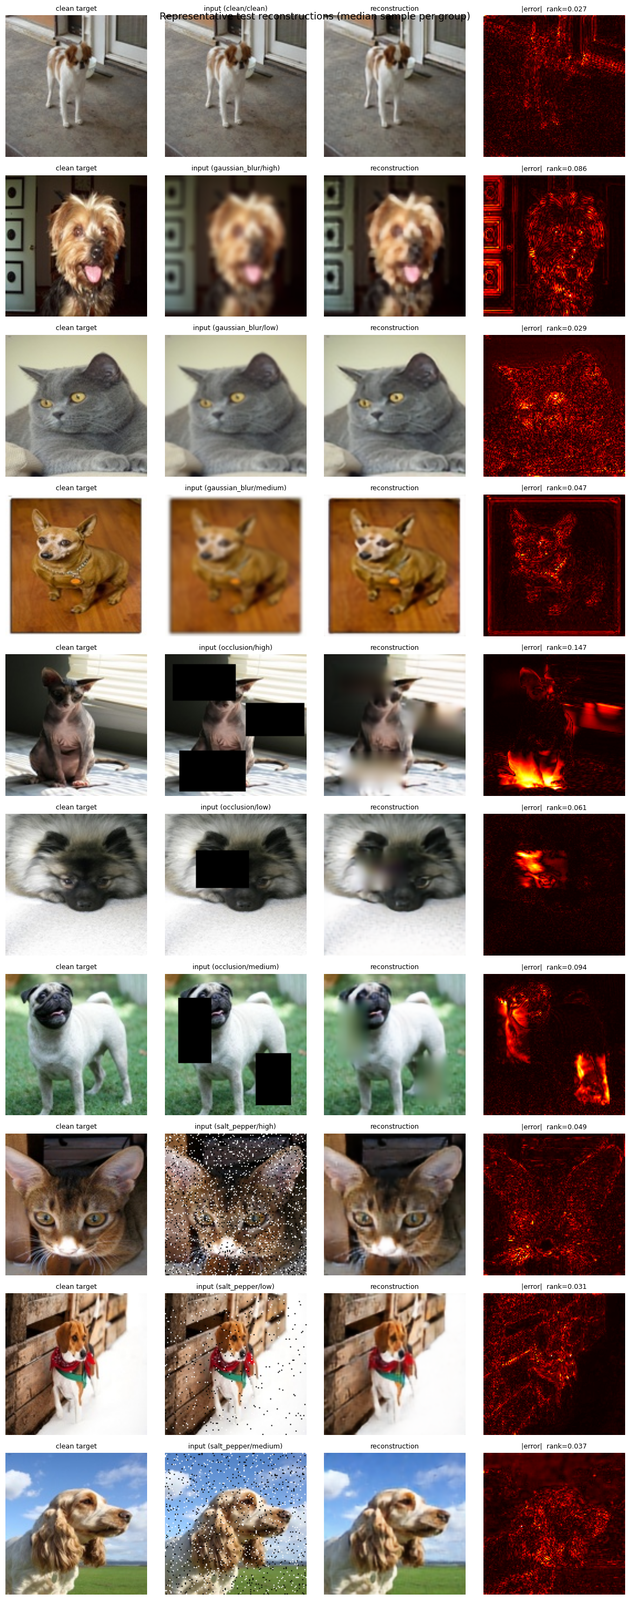
\includegraphics[width=0.94\columnwidth]{task1/grid_representative.png}
\caption{Task 1 representative restorations supplied by the evaluation pipeline. Each grid should be interpreted as a comparison of target, corrupted input, reconstruction, and residual error.}
\label{fig:task1representative}
\end{figure}

\begin{figure}[t]
\centering
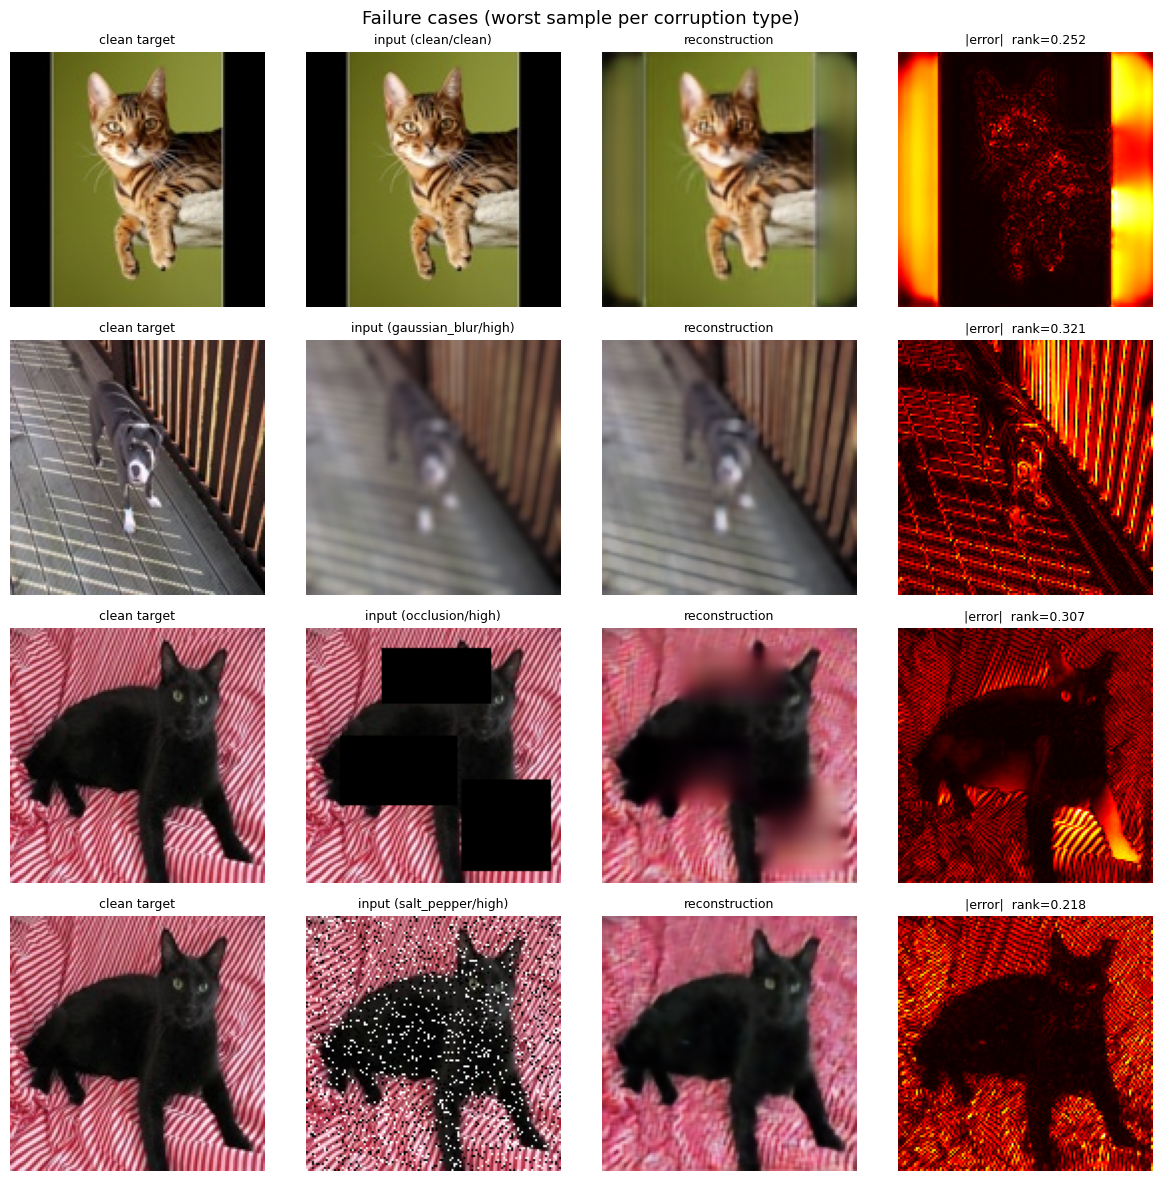
\includegraphics[width=\columnwidth]{task1/grid_failures.png}
\caption{Task 1 failure cases. These examples are important because aggregate SSIM can conceal localized hallucination or under-restoration.}
\label{fig:task1failures}
\end{figure}

\begin{figure*}[t]
\centering
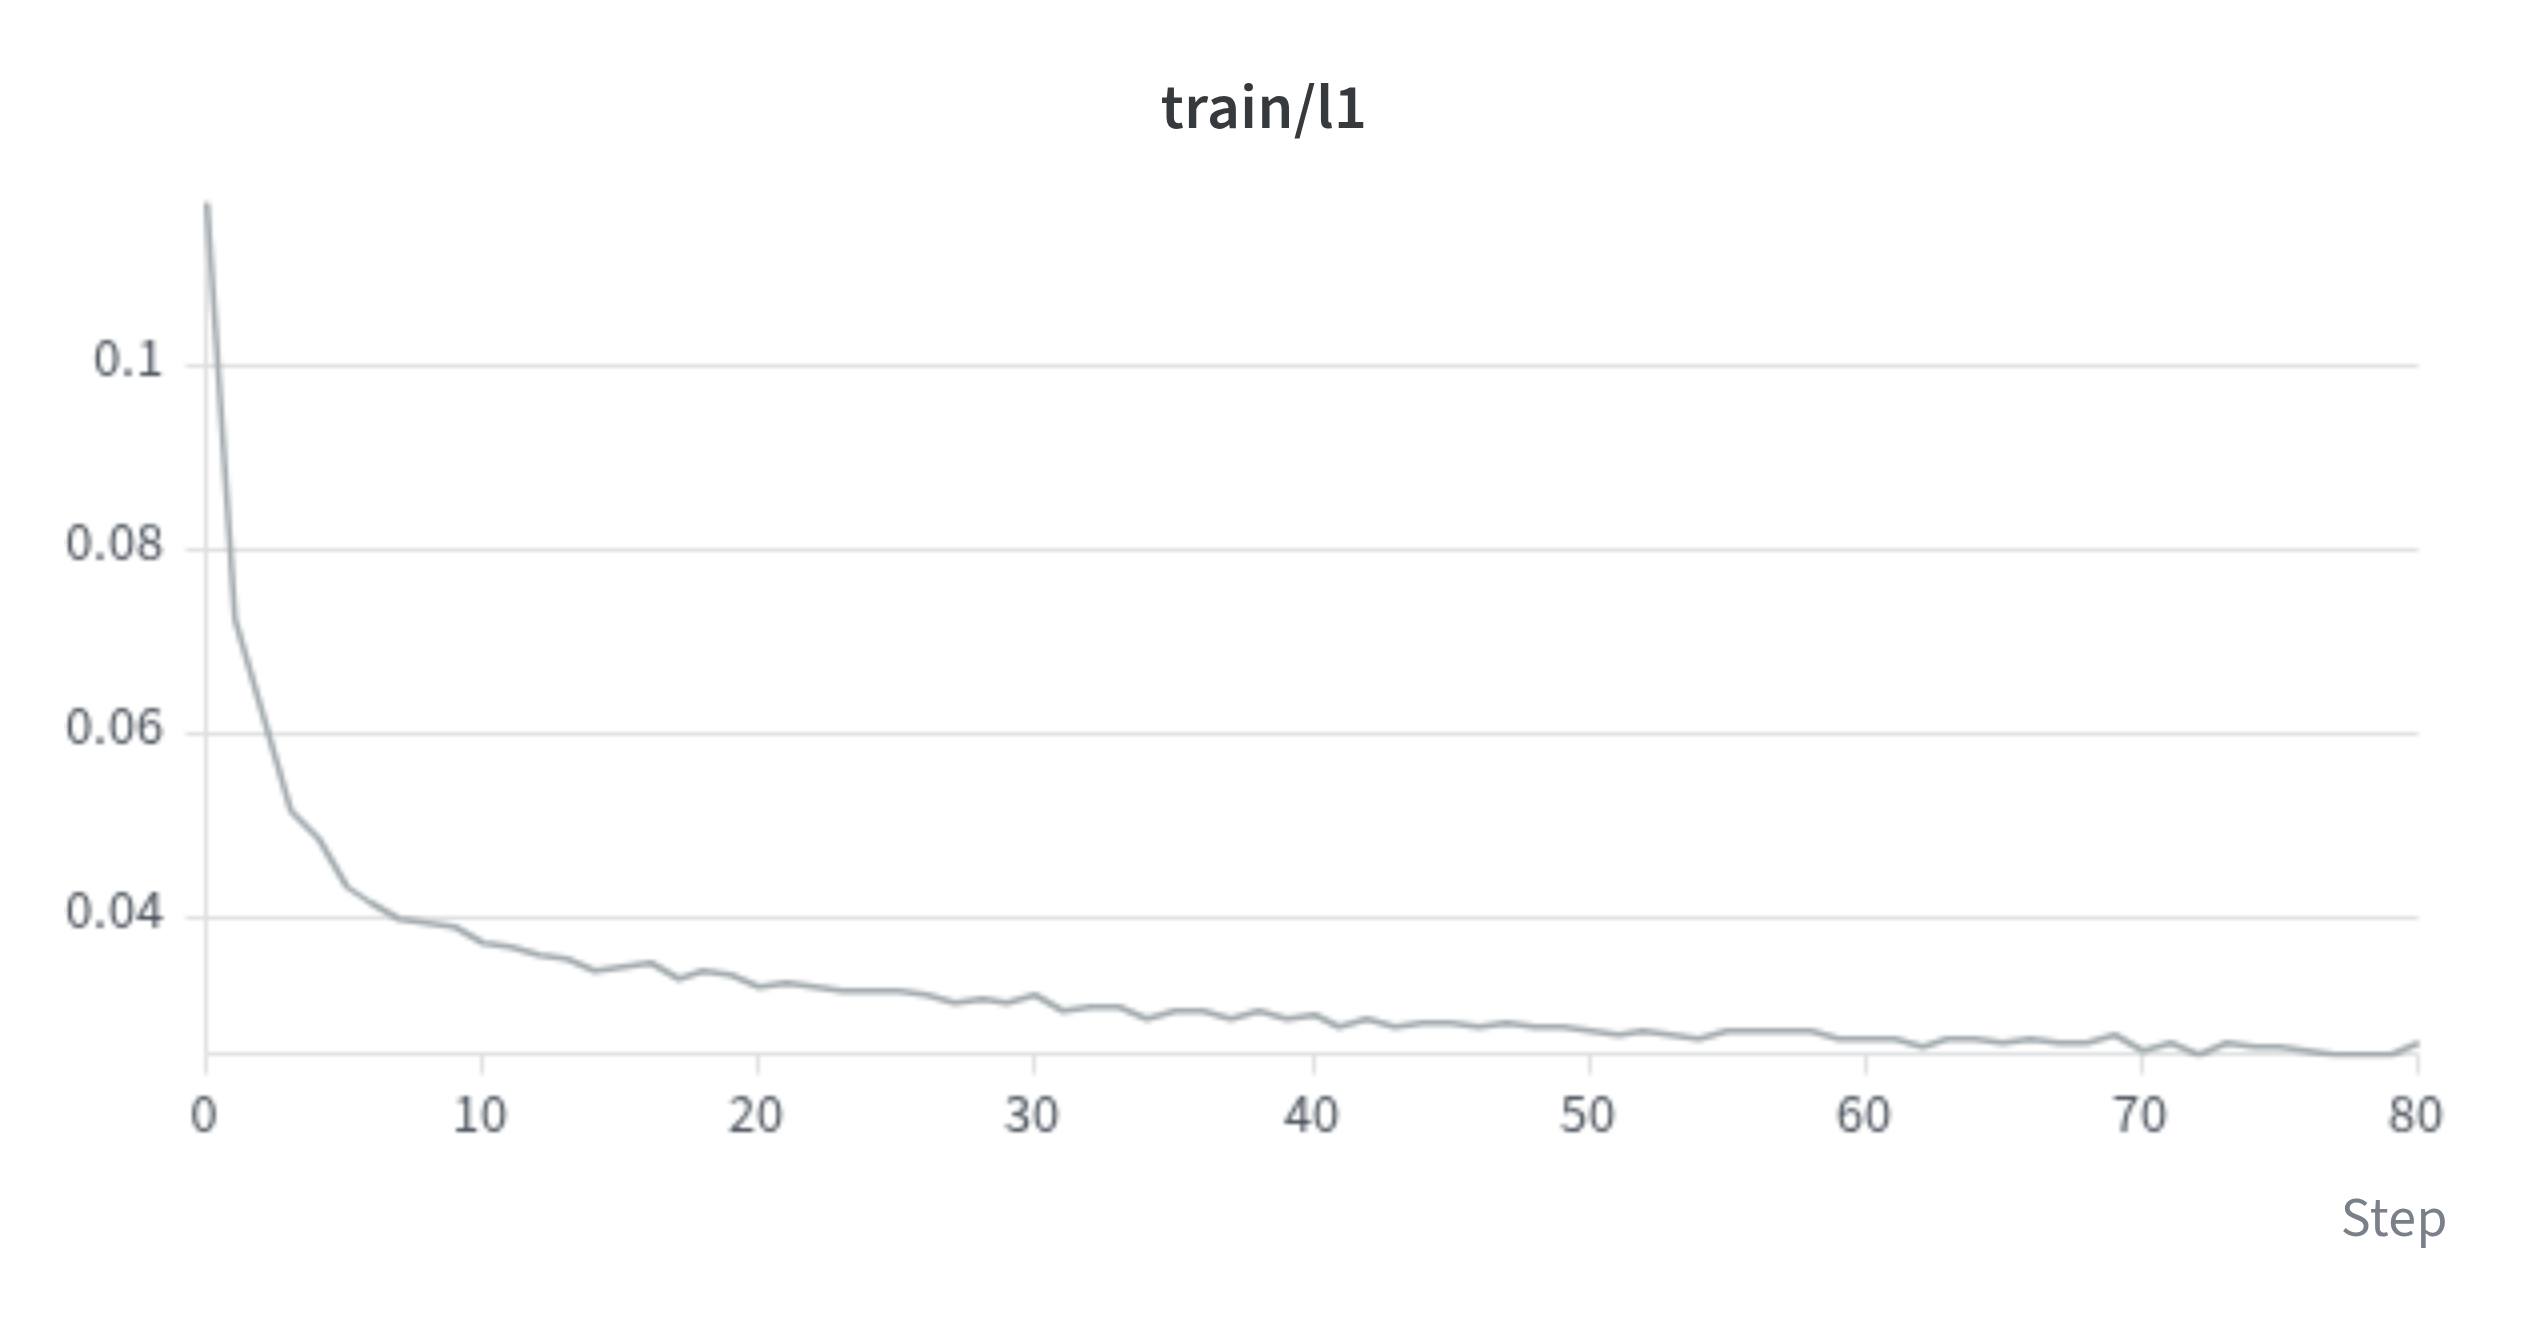
\includegraphics[width=0.31\textwidth]{task1_final_train_l1.png}
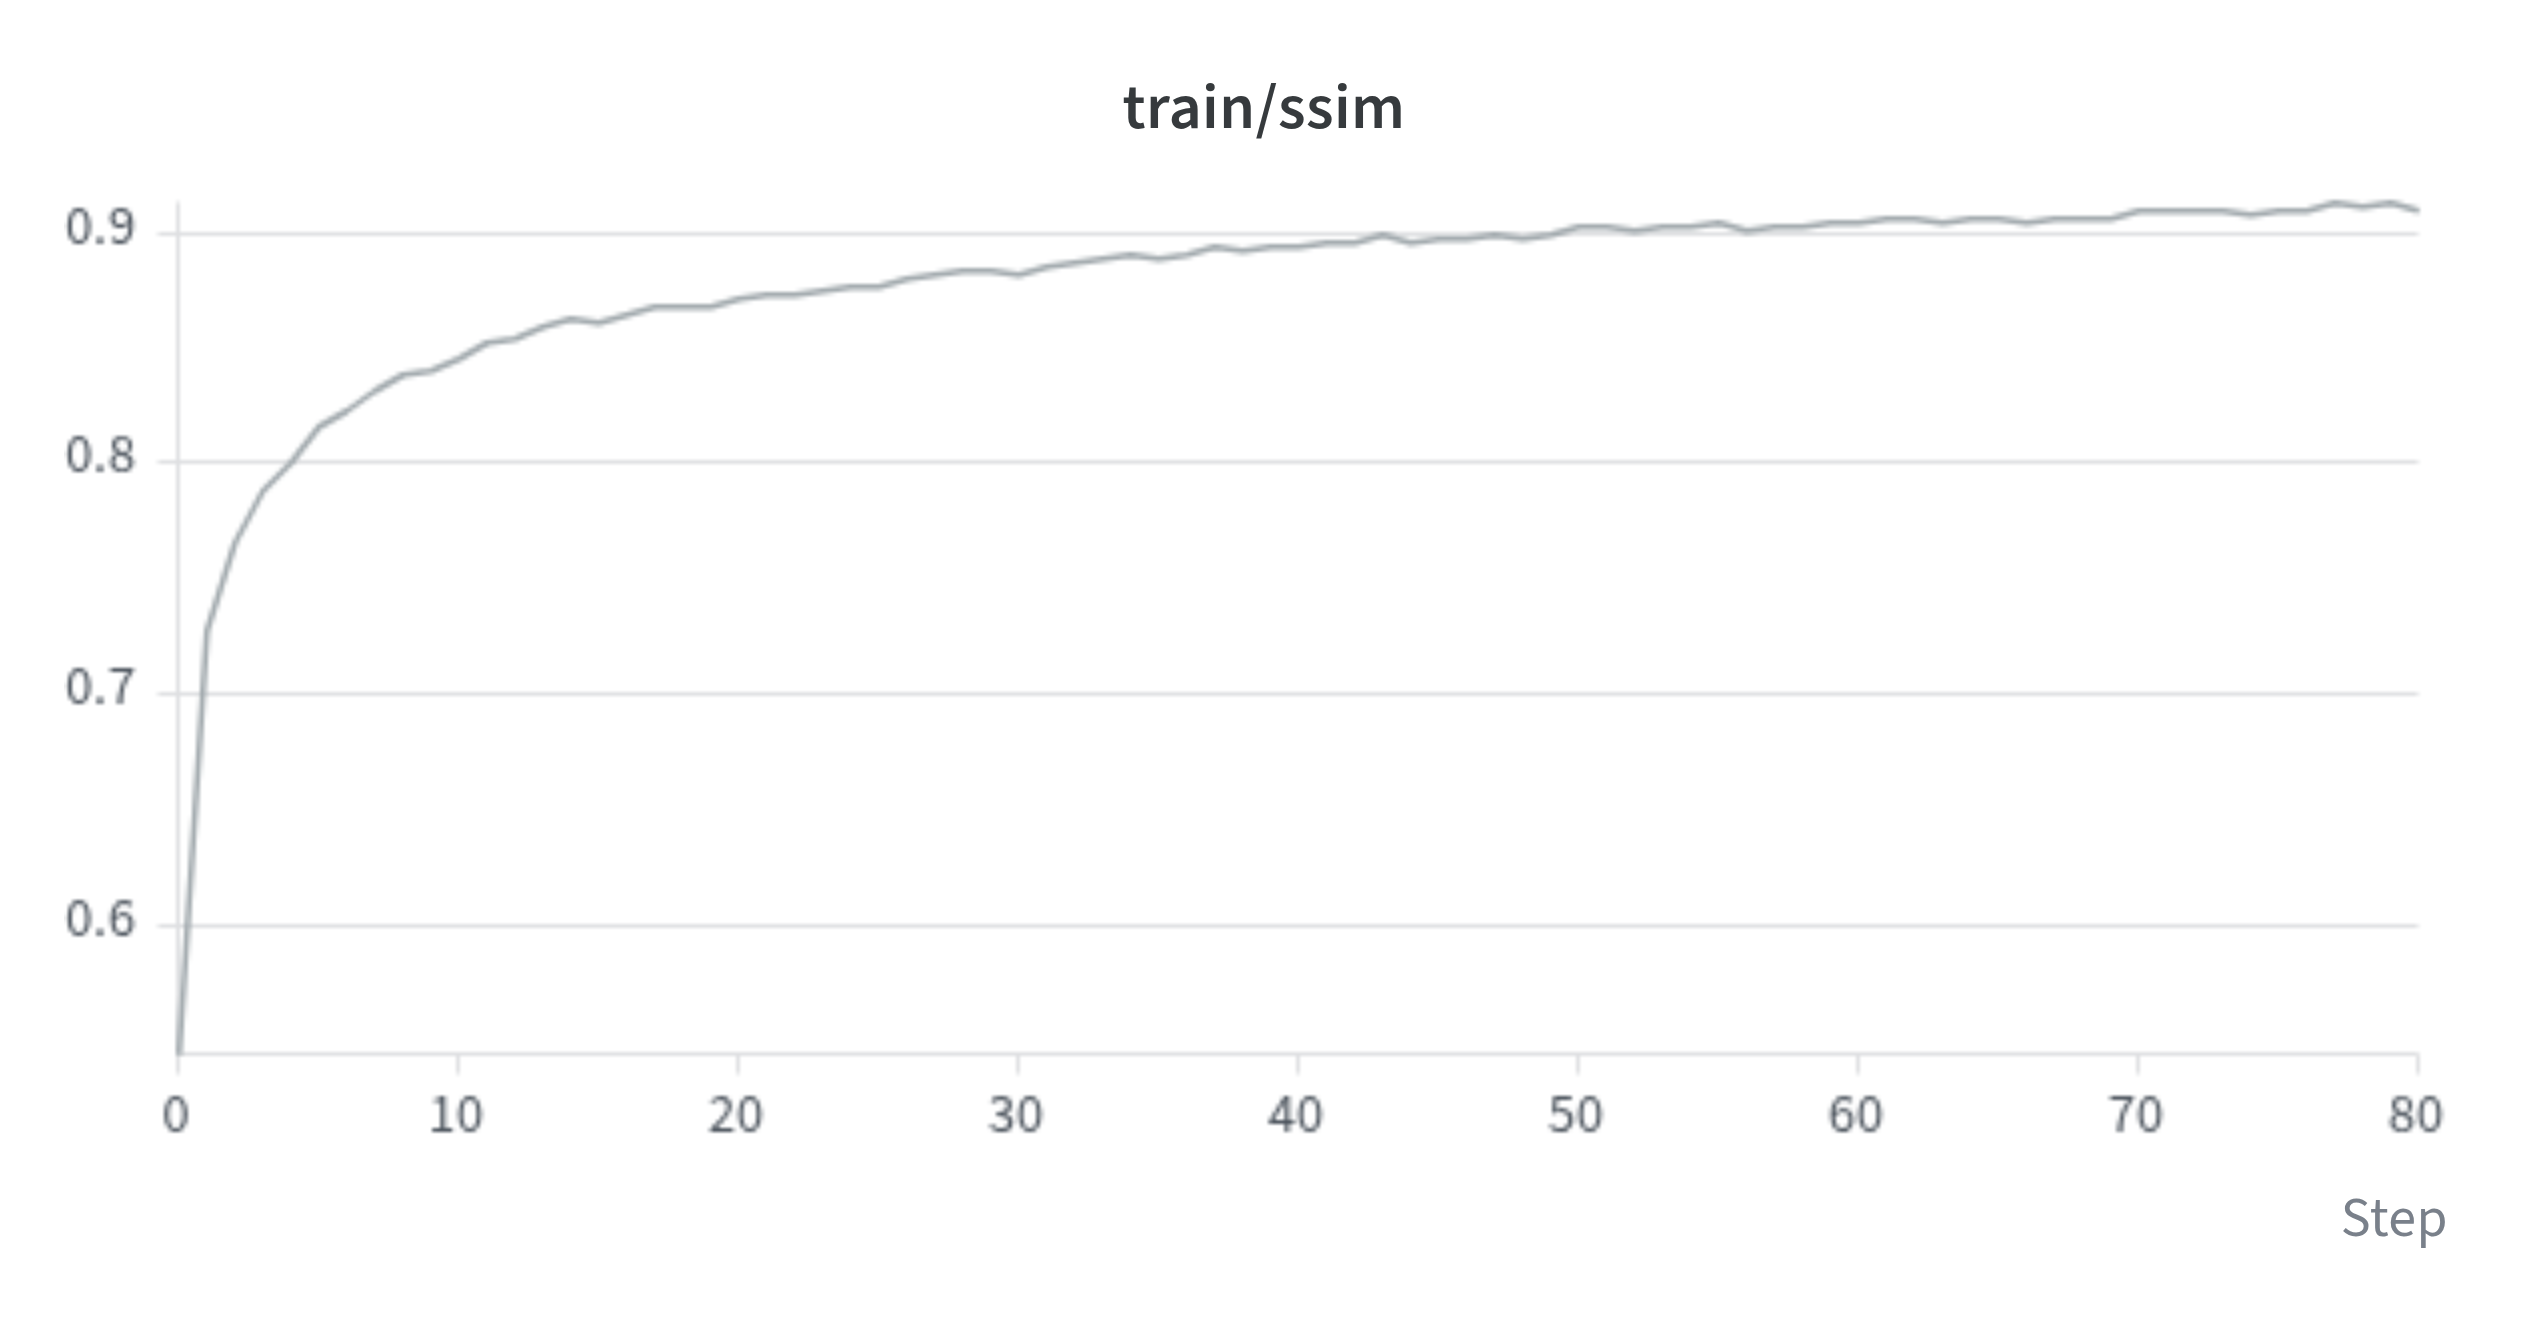
\includegraphics[width=0.31\textwidth]{task1_final_train_ssim.png}
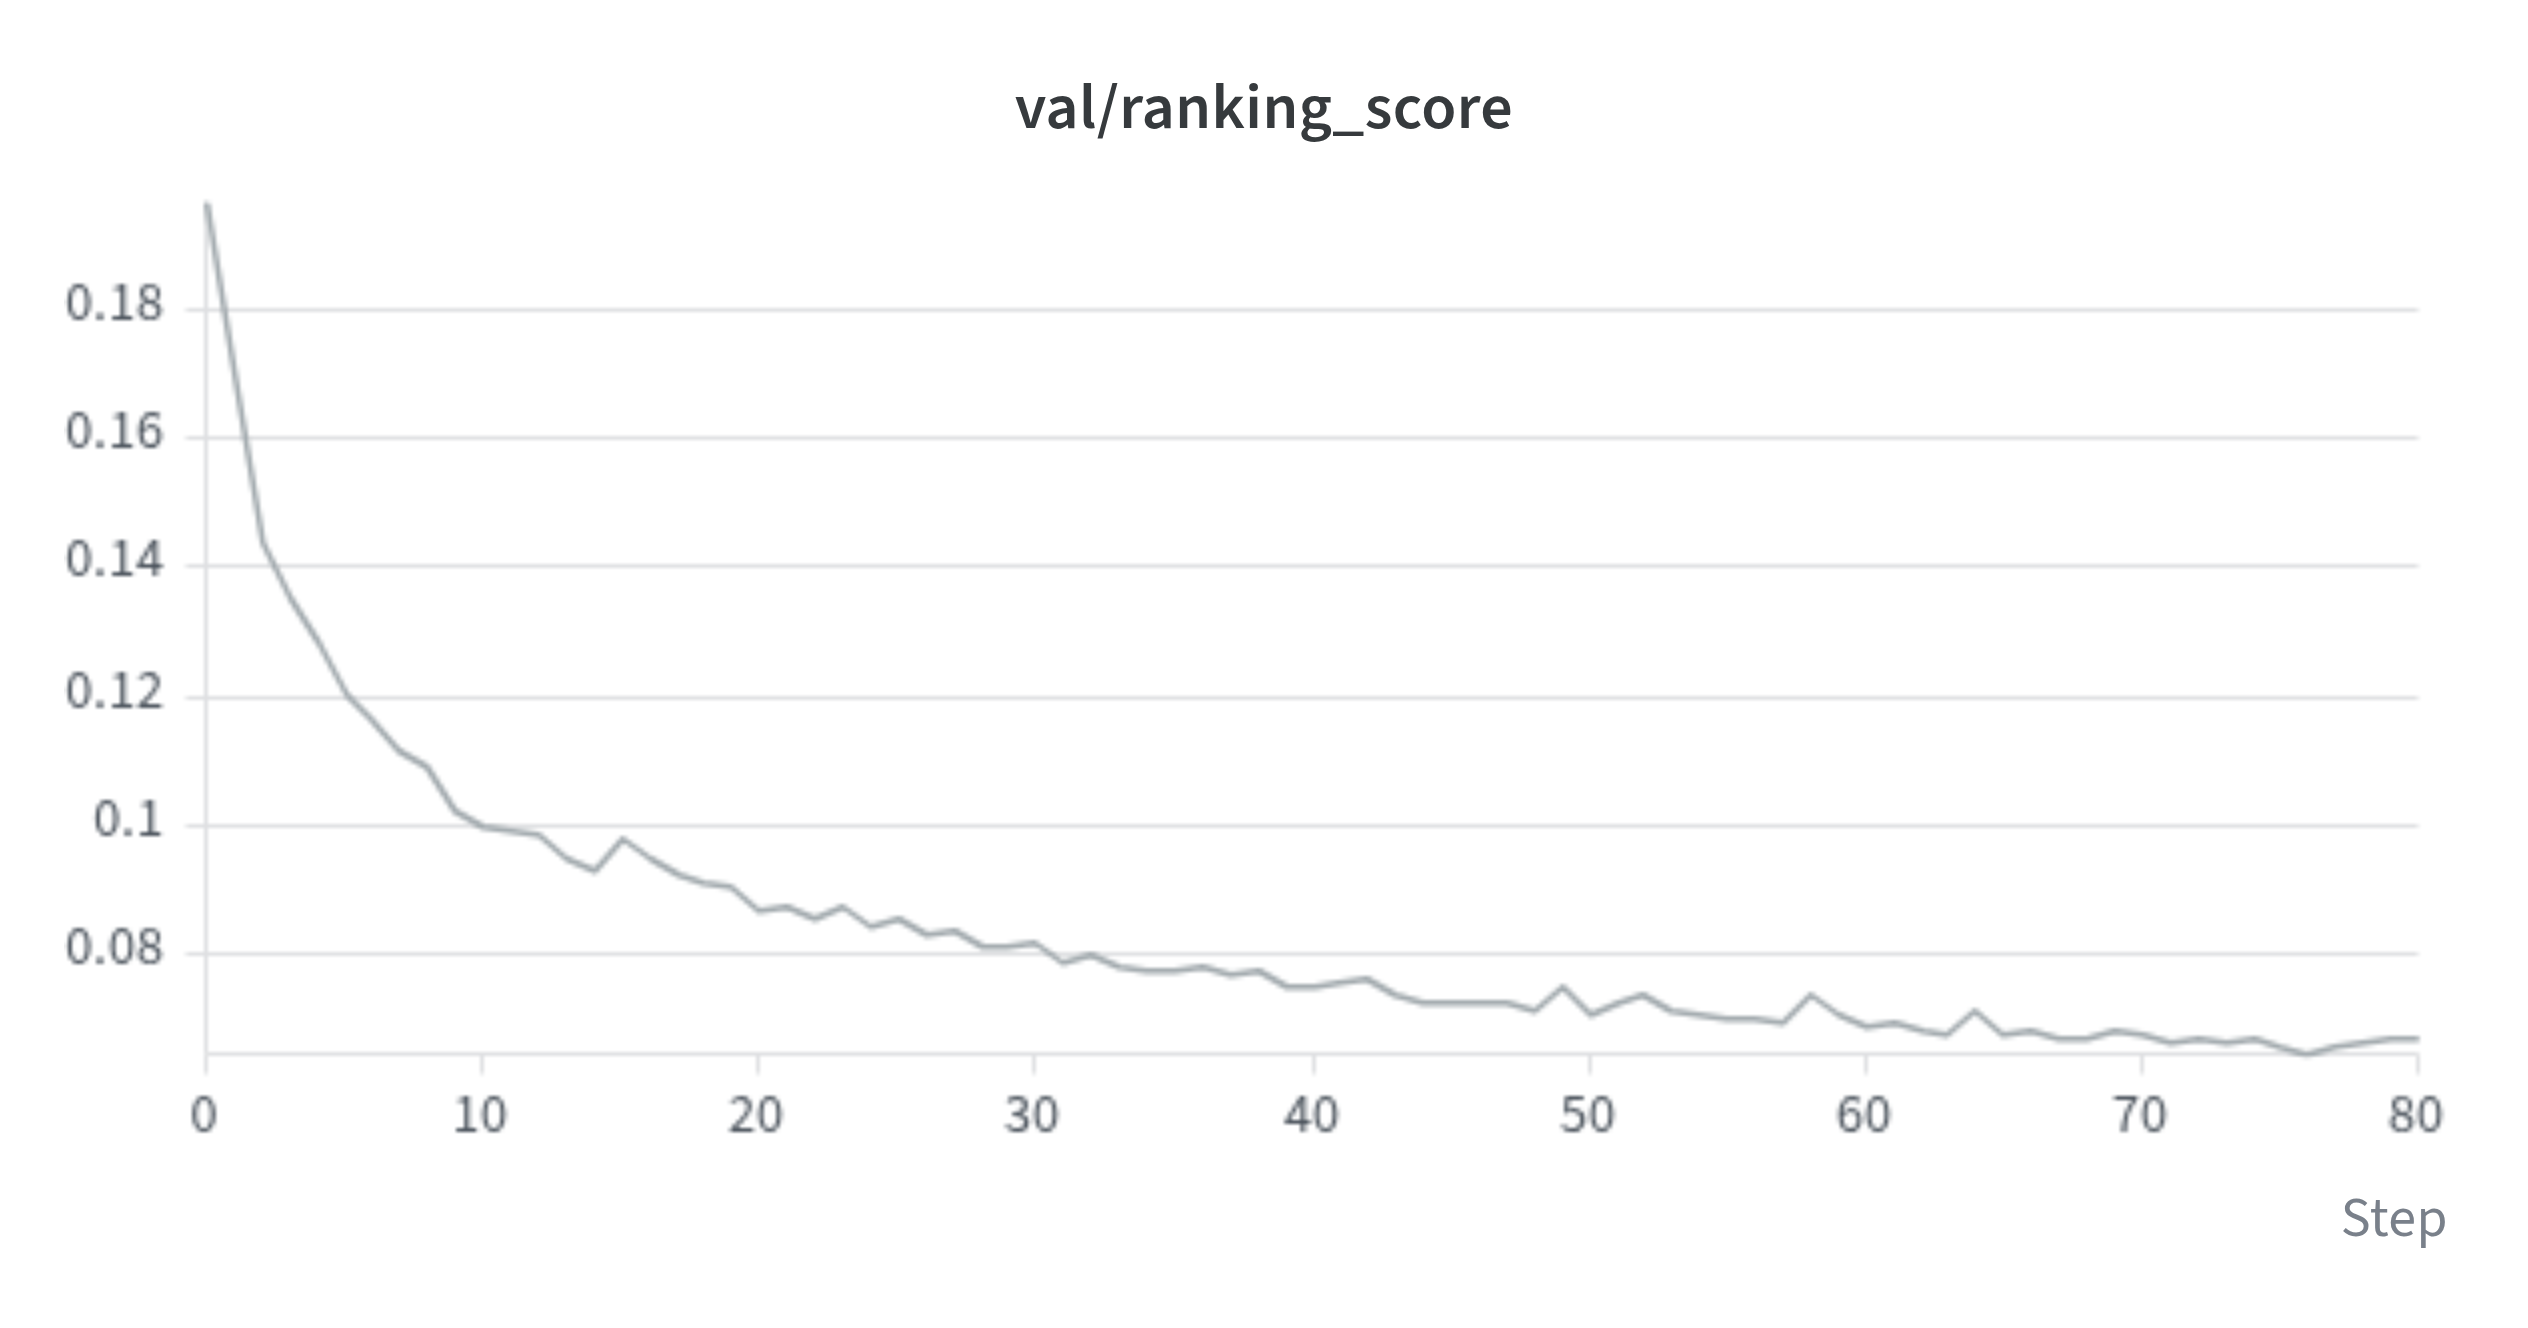
\includegraphics[width=0.31\textwidth]{task1_final_val_ranking_score.png}
\caption{Task 1 training and validation traces exported from the local W\&B records. Training L1 decreases, training SSIM increases, and the validation ranking score decreases rapidly before entering a slower-improvement regime. The separation between training and validation should be interpreted together with the final test table rather than as evidence of perfect generalization.}
\label{fig:task1curves}
\end{figure*}

\section{Task 2: Hard-Routed Specialists}
\subsection{Classifier and routing model}
The classifier predicts $p=C(\tilde{x})=[p_{clean},p_{salt},p_{blur},p_{occ}]$ using multiclass cross-entropy. The predicted class is $r=\arg\max_k p_k$. Clean images use an identity bypass; the other classes select independently trained salt-pepper, blur, or occlusion specialists. The predicted operational system is evaluated separately from oracle routing, where the known manifest label chooses the specialist.

The classifier search varies learning rate $\in[10^{-4},10^{-2}]$, batch size $\in\{16,32,64\}$, base channels $\in\{16,32,48,64\}$, dropout $\in[0,0.5]$, and weight decay $\in[10^{-5},10^{-2}]$. A shared specialist search varies learning rate, latent dimension $\in\{128,256,512\}$, base channels $\in\{16,32,48\}$, batch size, $\alpha$, weight decay, and skip count. Optuna uses a TPE sampler seeded at 42 and median pruning.

\subsection{Results}
\begin{table}[t]
\caption{Task 2 classifier results on the deterministic test manifest.}
\label{tab:classifier}
\centering
\begin{tabular}{lc}
\toprule
Metric & Value\\
\midrule
Accuracy & 0.99210\\
Macro precision & 0.98539\\
Macro recall & 0.98919\\
Macro F1 & 0.98725\\
\bottomrule
\end{tabular}
\end{table}

Per-class F1 is 0.96284 for clean, 0.99873 for salt-pepper, 0.99198 for Gaussian blur, and 0.99546 for occlusion. The lower clean score is consistent with clean inputs being visually close to low-severity corruption and therefore less separable than strongly corrupted inputs.

\begin{table}[t]
\caption{Task 2 end-to-end restoration results.}
\label{tab:task2restoration}
\centering
\begin{tabular}{lccc}
\toprule
Routing & L1 & SSIM & $n$\\
\midrule
Oracle & 0.05579 & 0.76271 & 36,690\\
Predicted & 0.05574 & 0.76287 & 36,690\\
\bottomrule
\end{tabular}
\end{table}

The nearly identical oracle and predicted aggregate scores indicate that classifier errors have limited aggregate impact in this test. This should not be interpreted as proof that misrouting is harmless: the worst-case grids show individual samples where a wrong expert creates a visibly inappropriate reconstruction.

\begin{figure}[t]
\centering
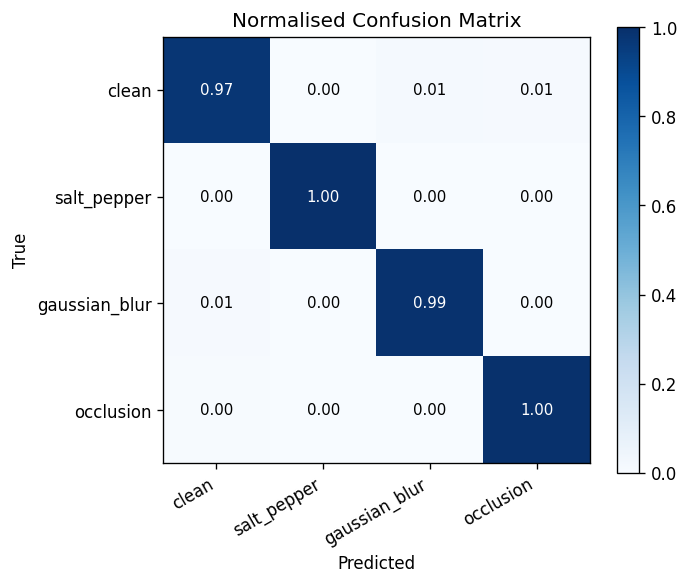
\includegraphics[width=\columnwidth]{task2/confusion_matrix.png}
\caption{Normalised Task 2 four-class confusion matrix. Diagonal concentration supports the high macro-F1 result, while the clean row contains the most visible confusion.}
\label{fig:confusion}
\end{figure}

\begin{figure}[t]
\centering
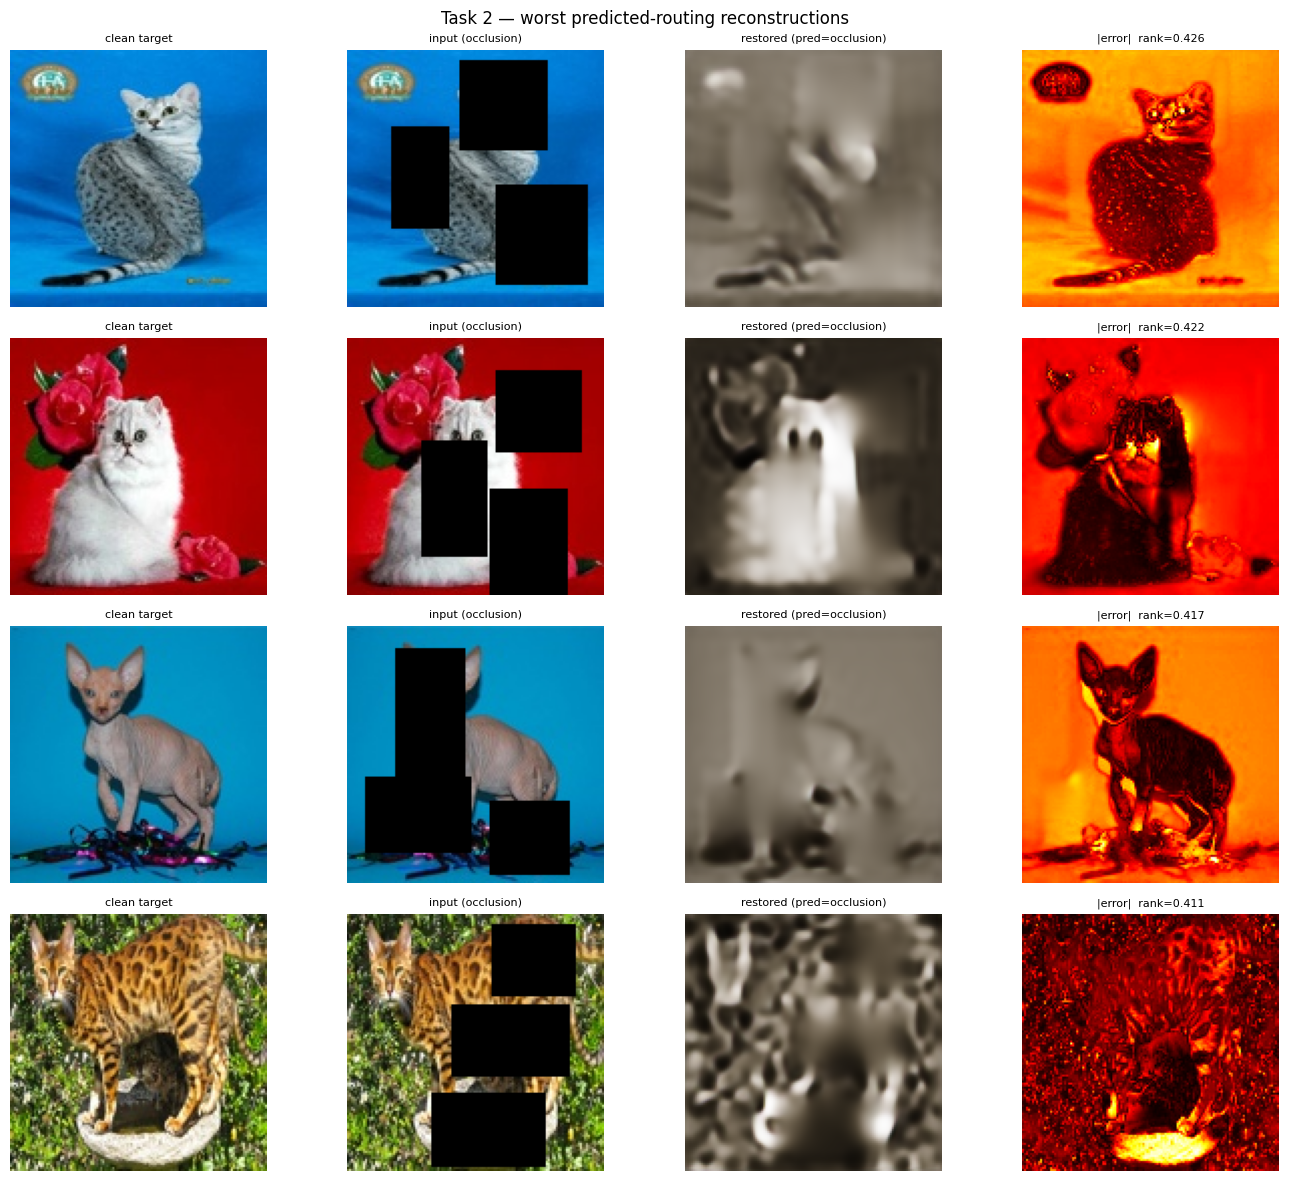
\includegraphics[width=\columnwidth]{task2/grid_worst_cases.png}
\caption{Task 2 worst misrouted cases. These cases expose failure modes that are not visible in aggregate accuracy.}
\label{fig:task2failures}
\end{figure}

\begin{figure*}[t]
\centering
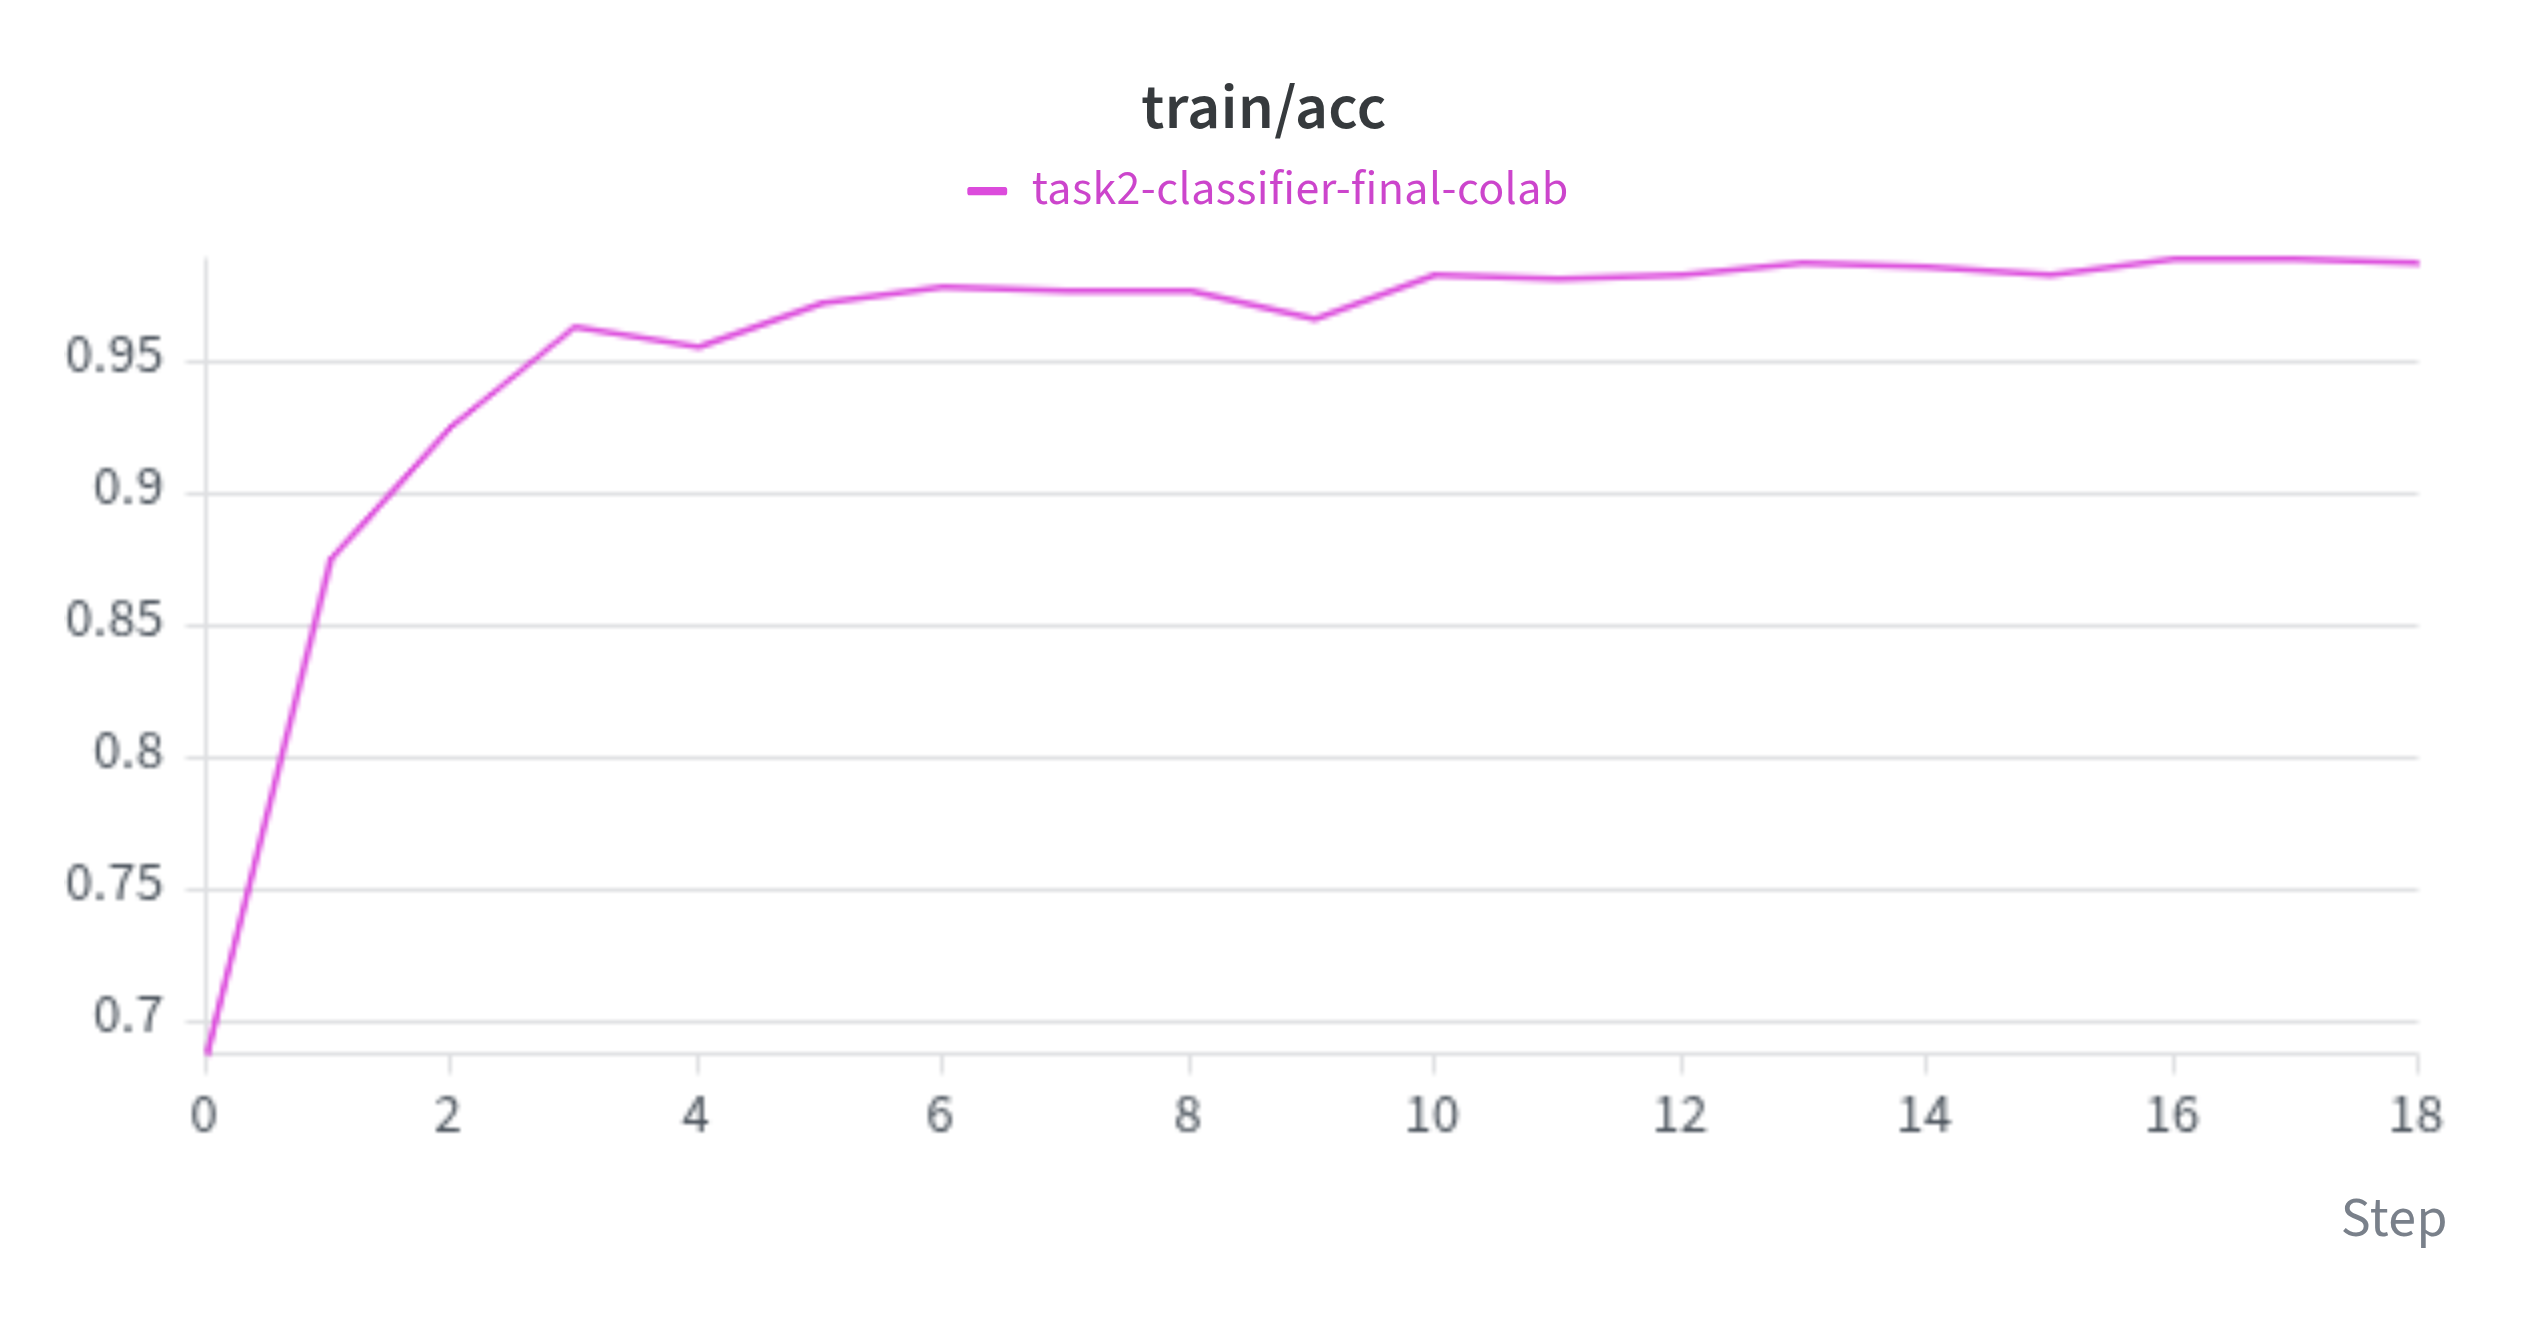
\includegraphics[width=0.24\textwidth]{classifier_train_acc.png}
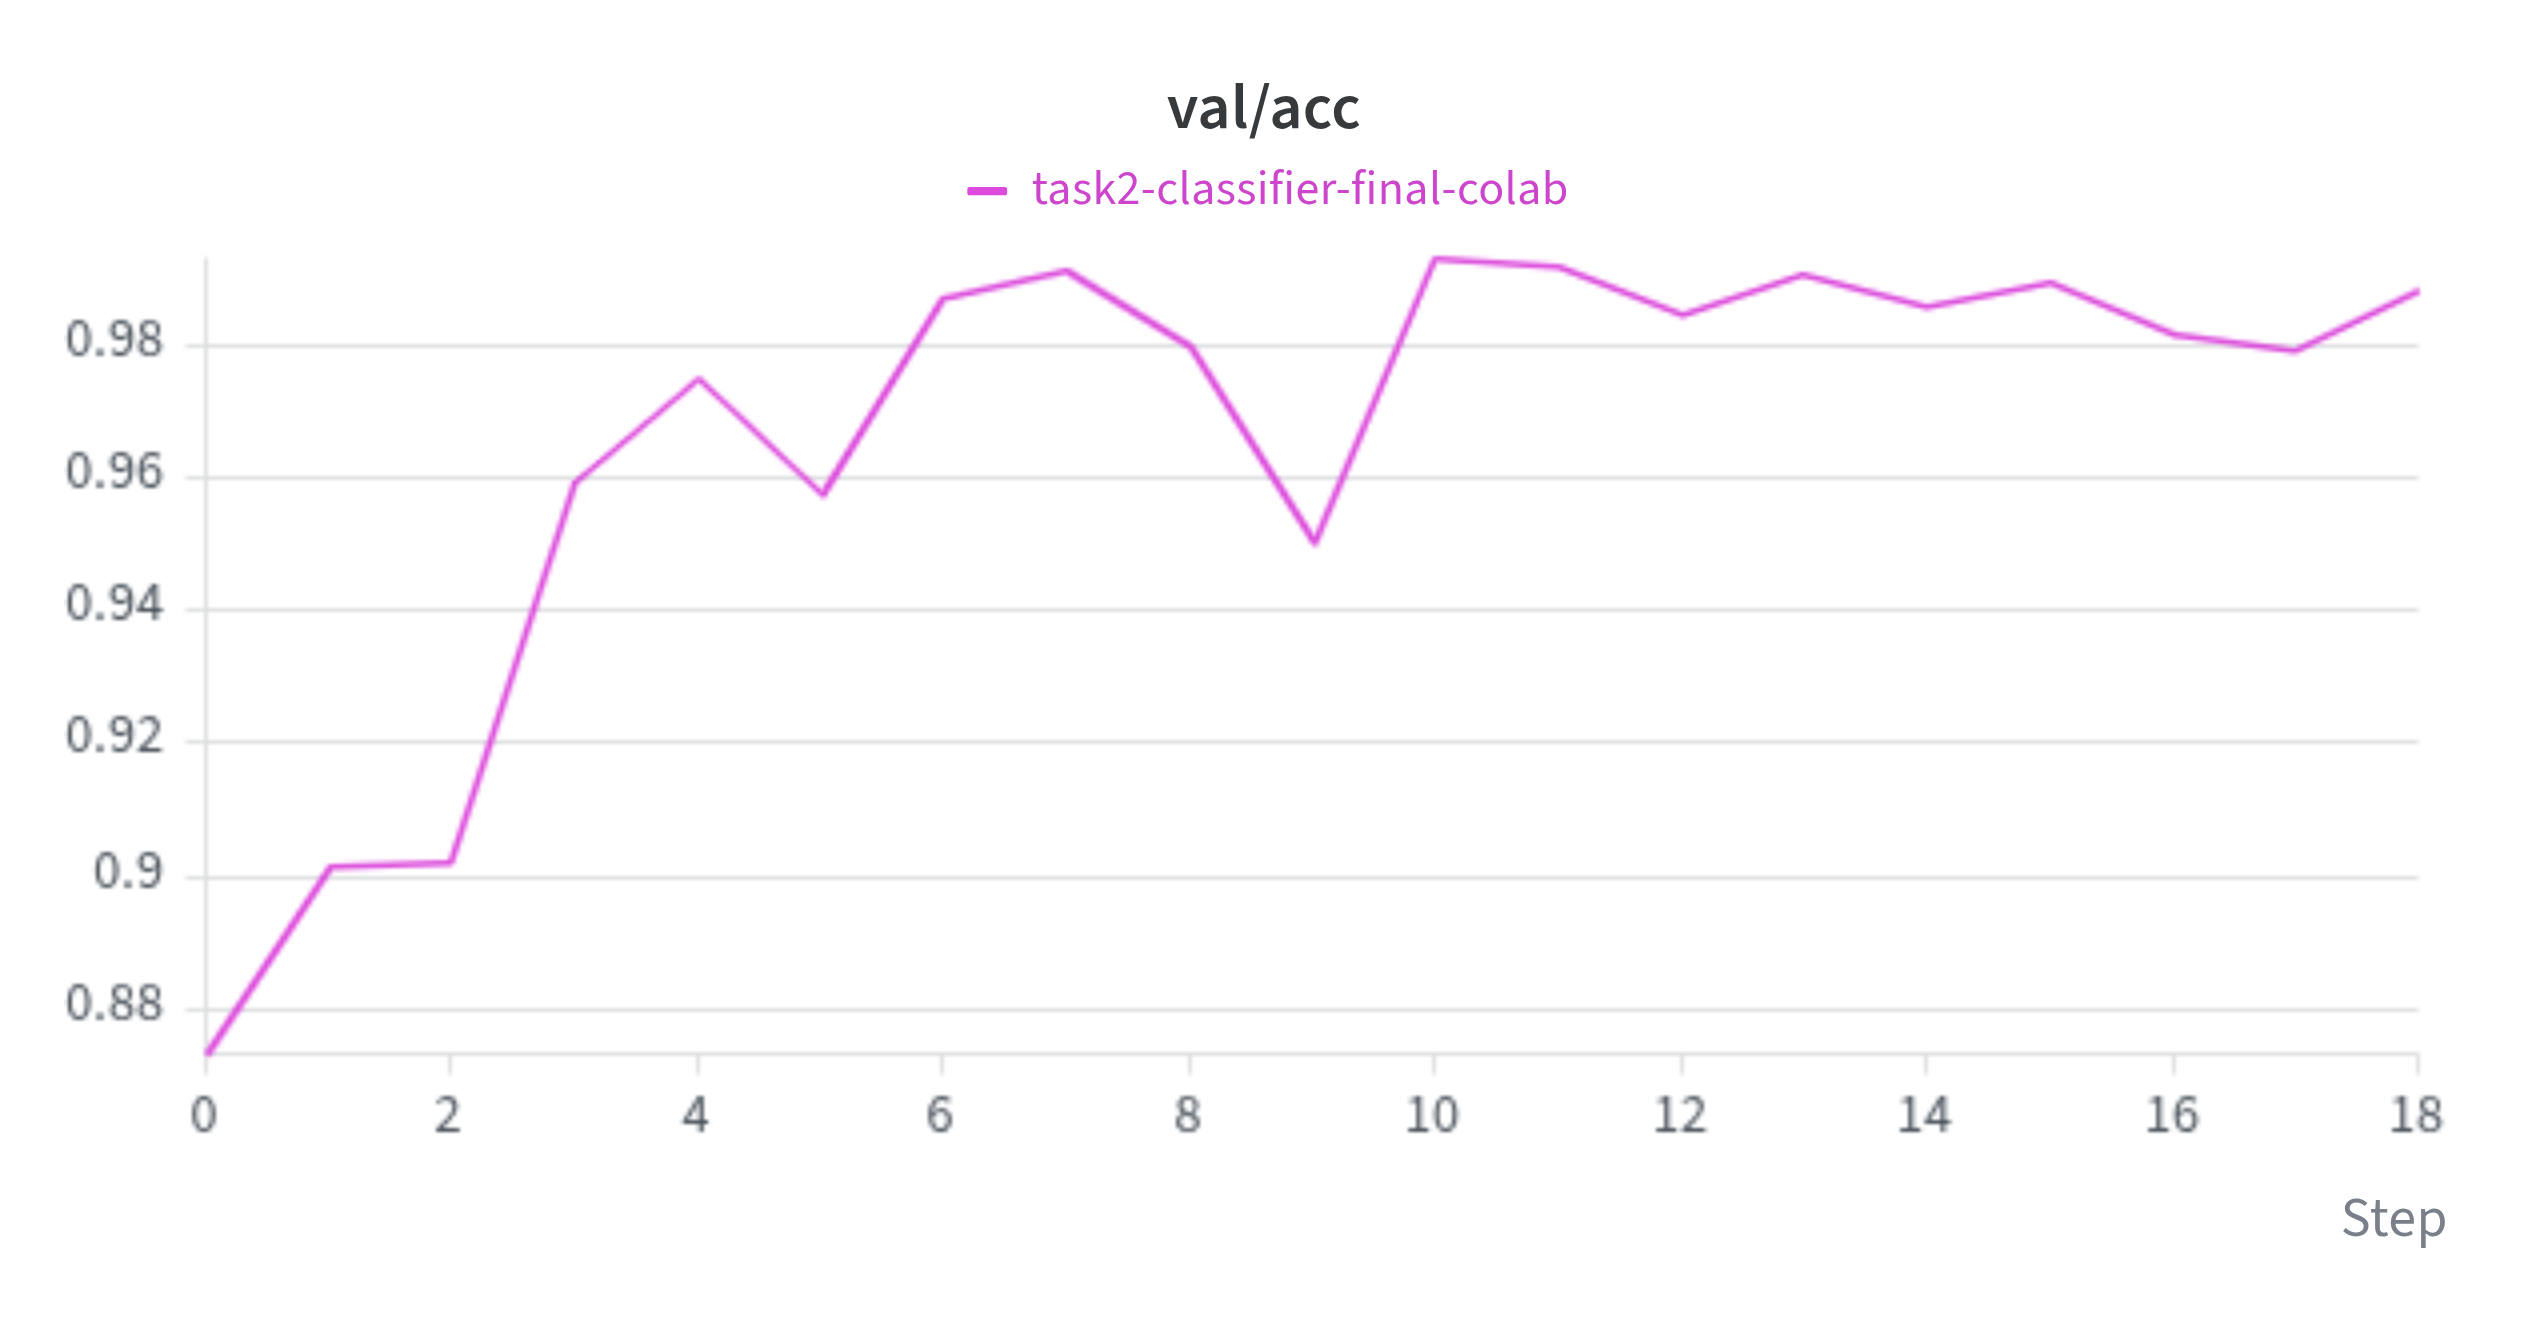
\includegraphics[width=0.24\textwidth]{classifier_val_acc.png}
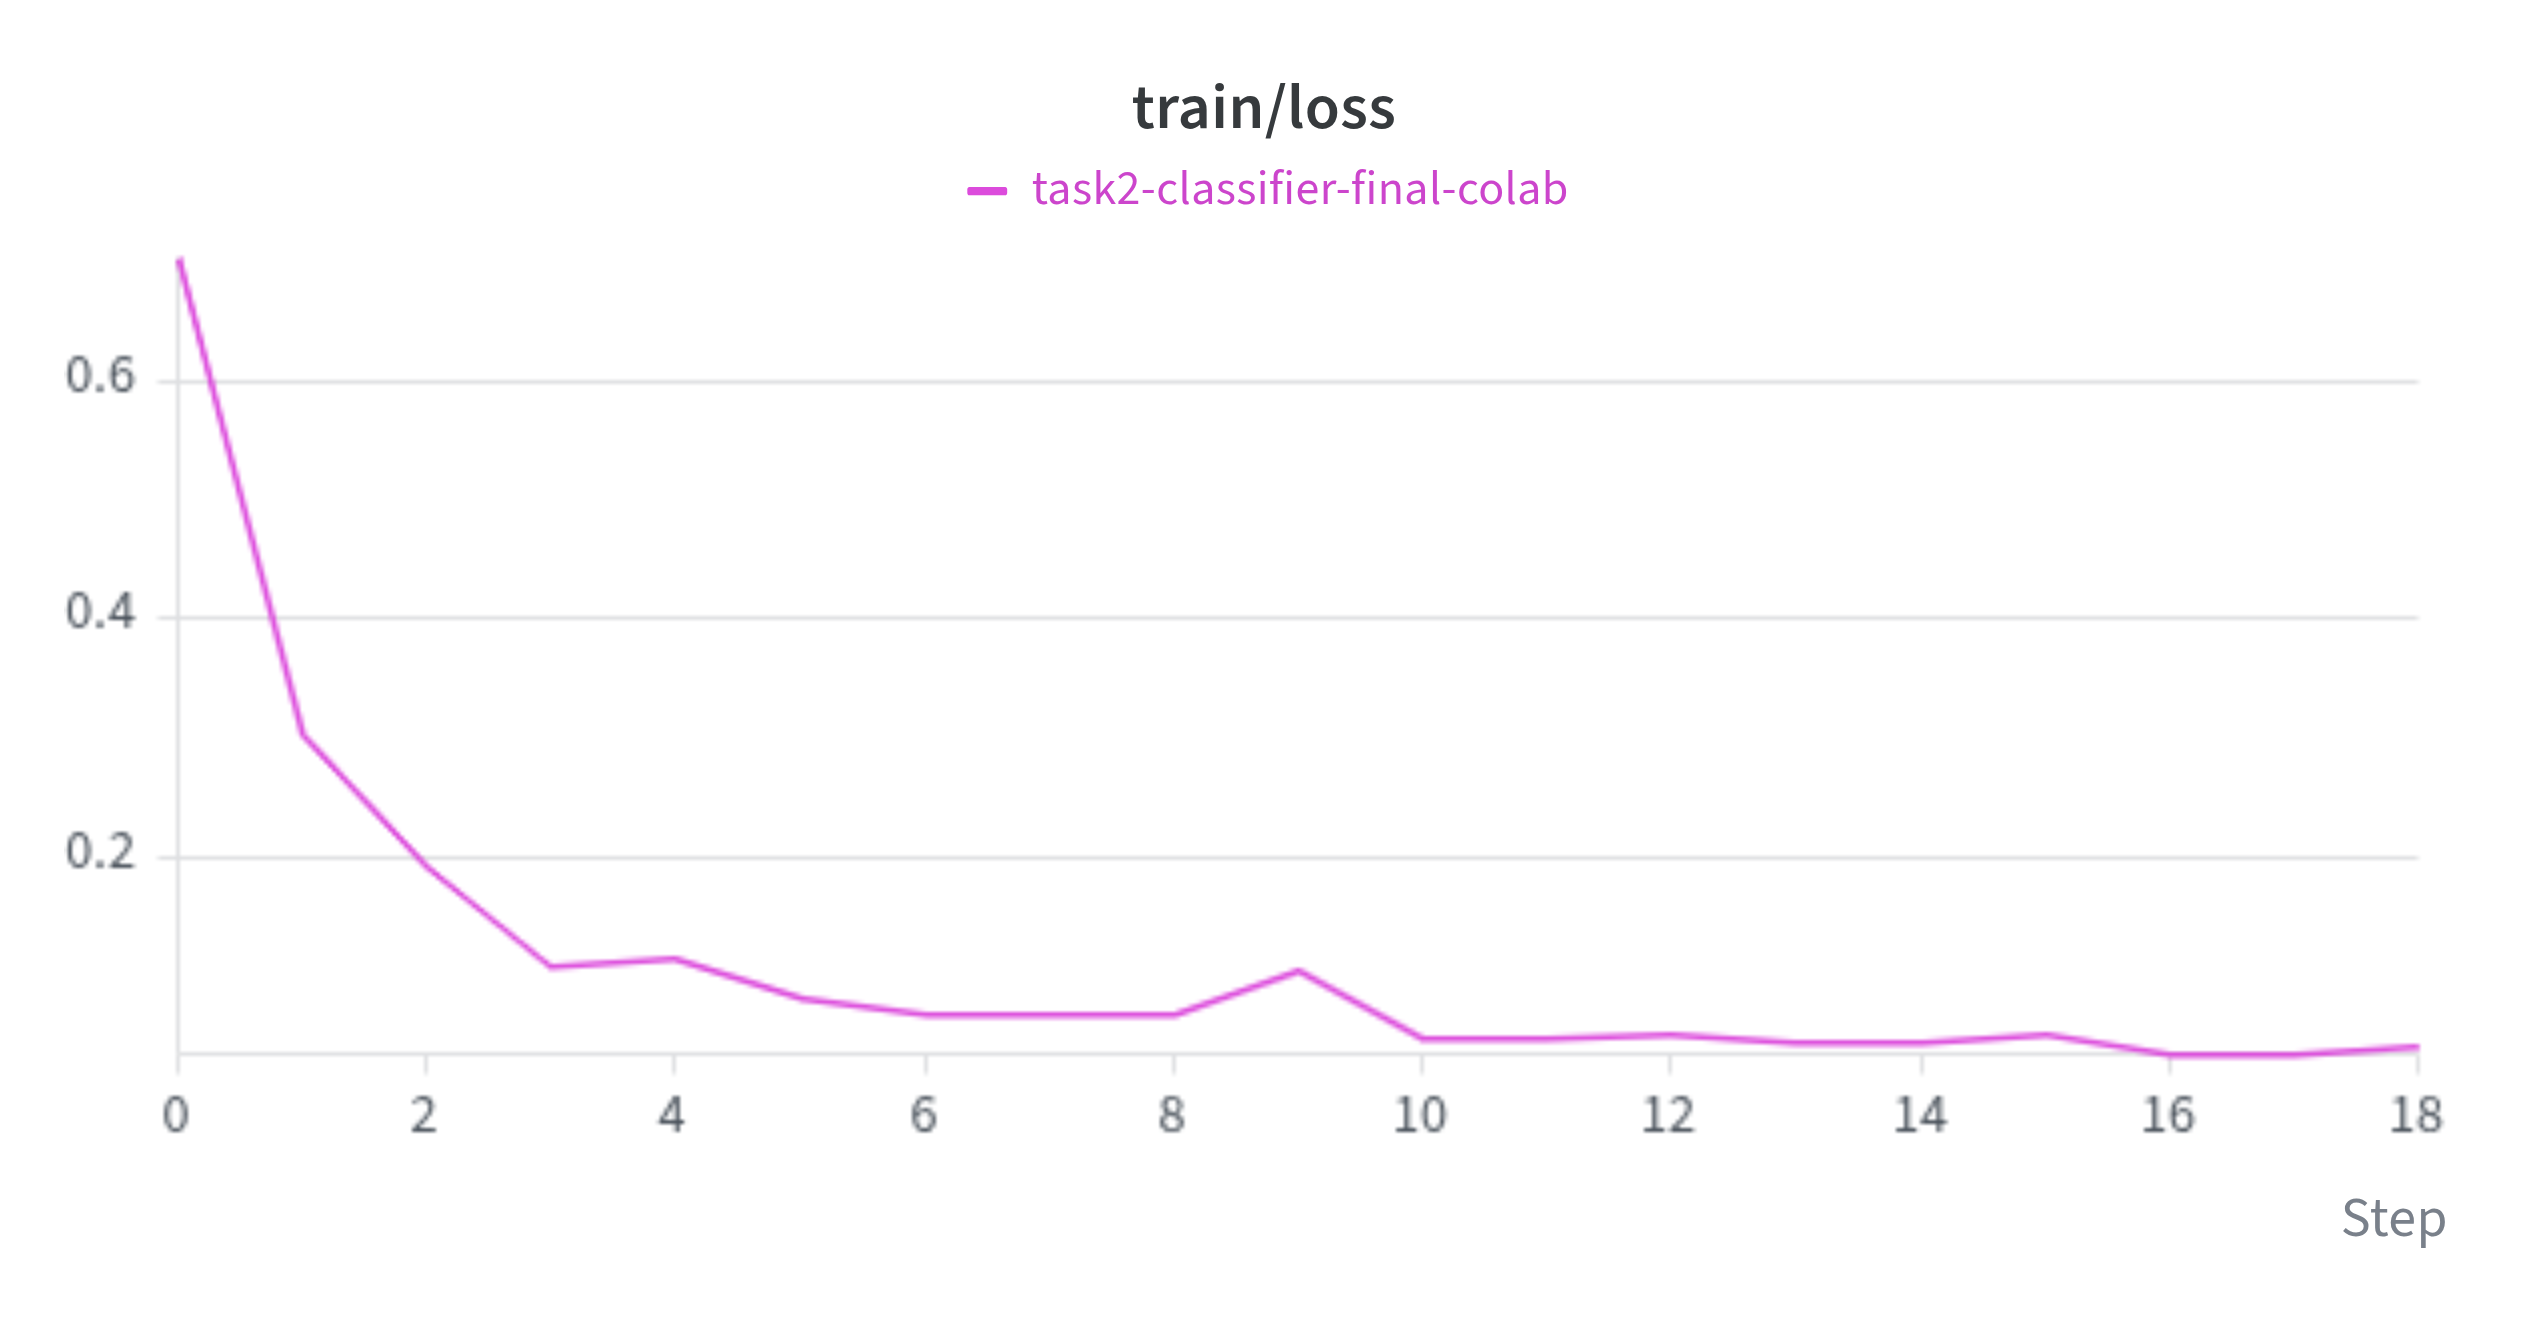
\includegraphics[width=0.24\textwidth]{classifier_train_loss.png}
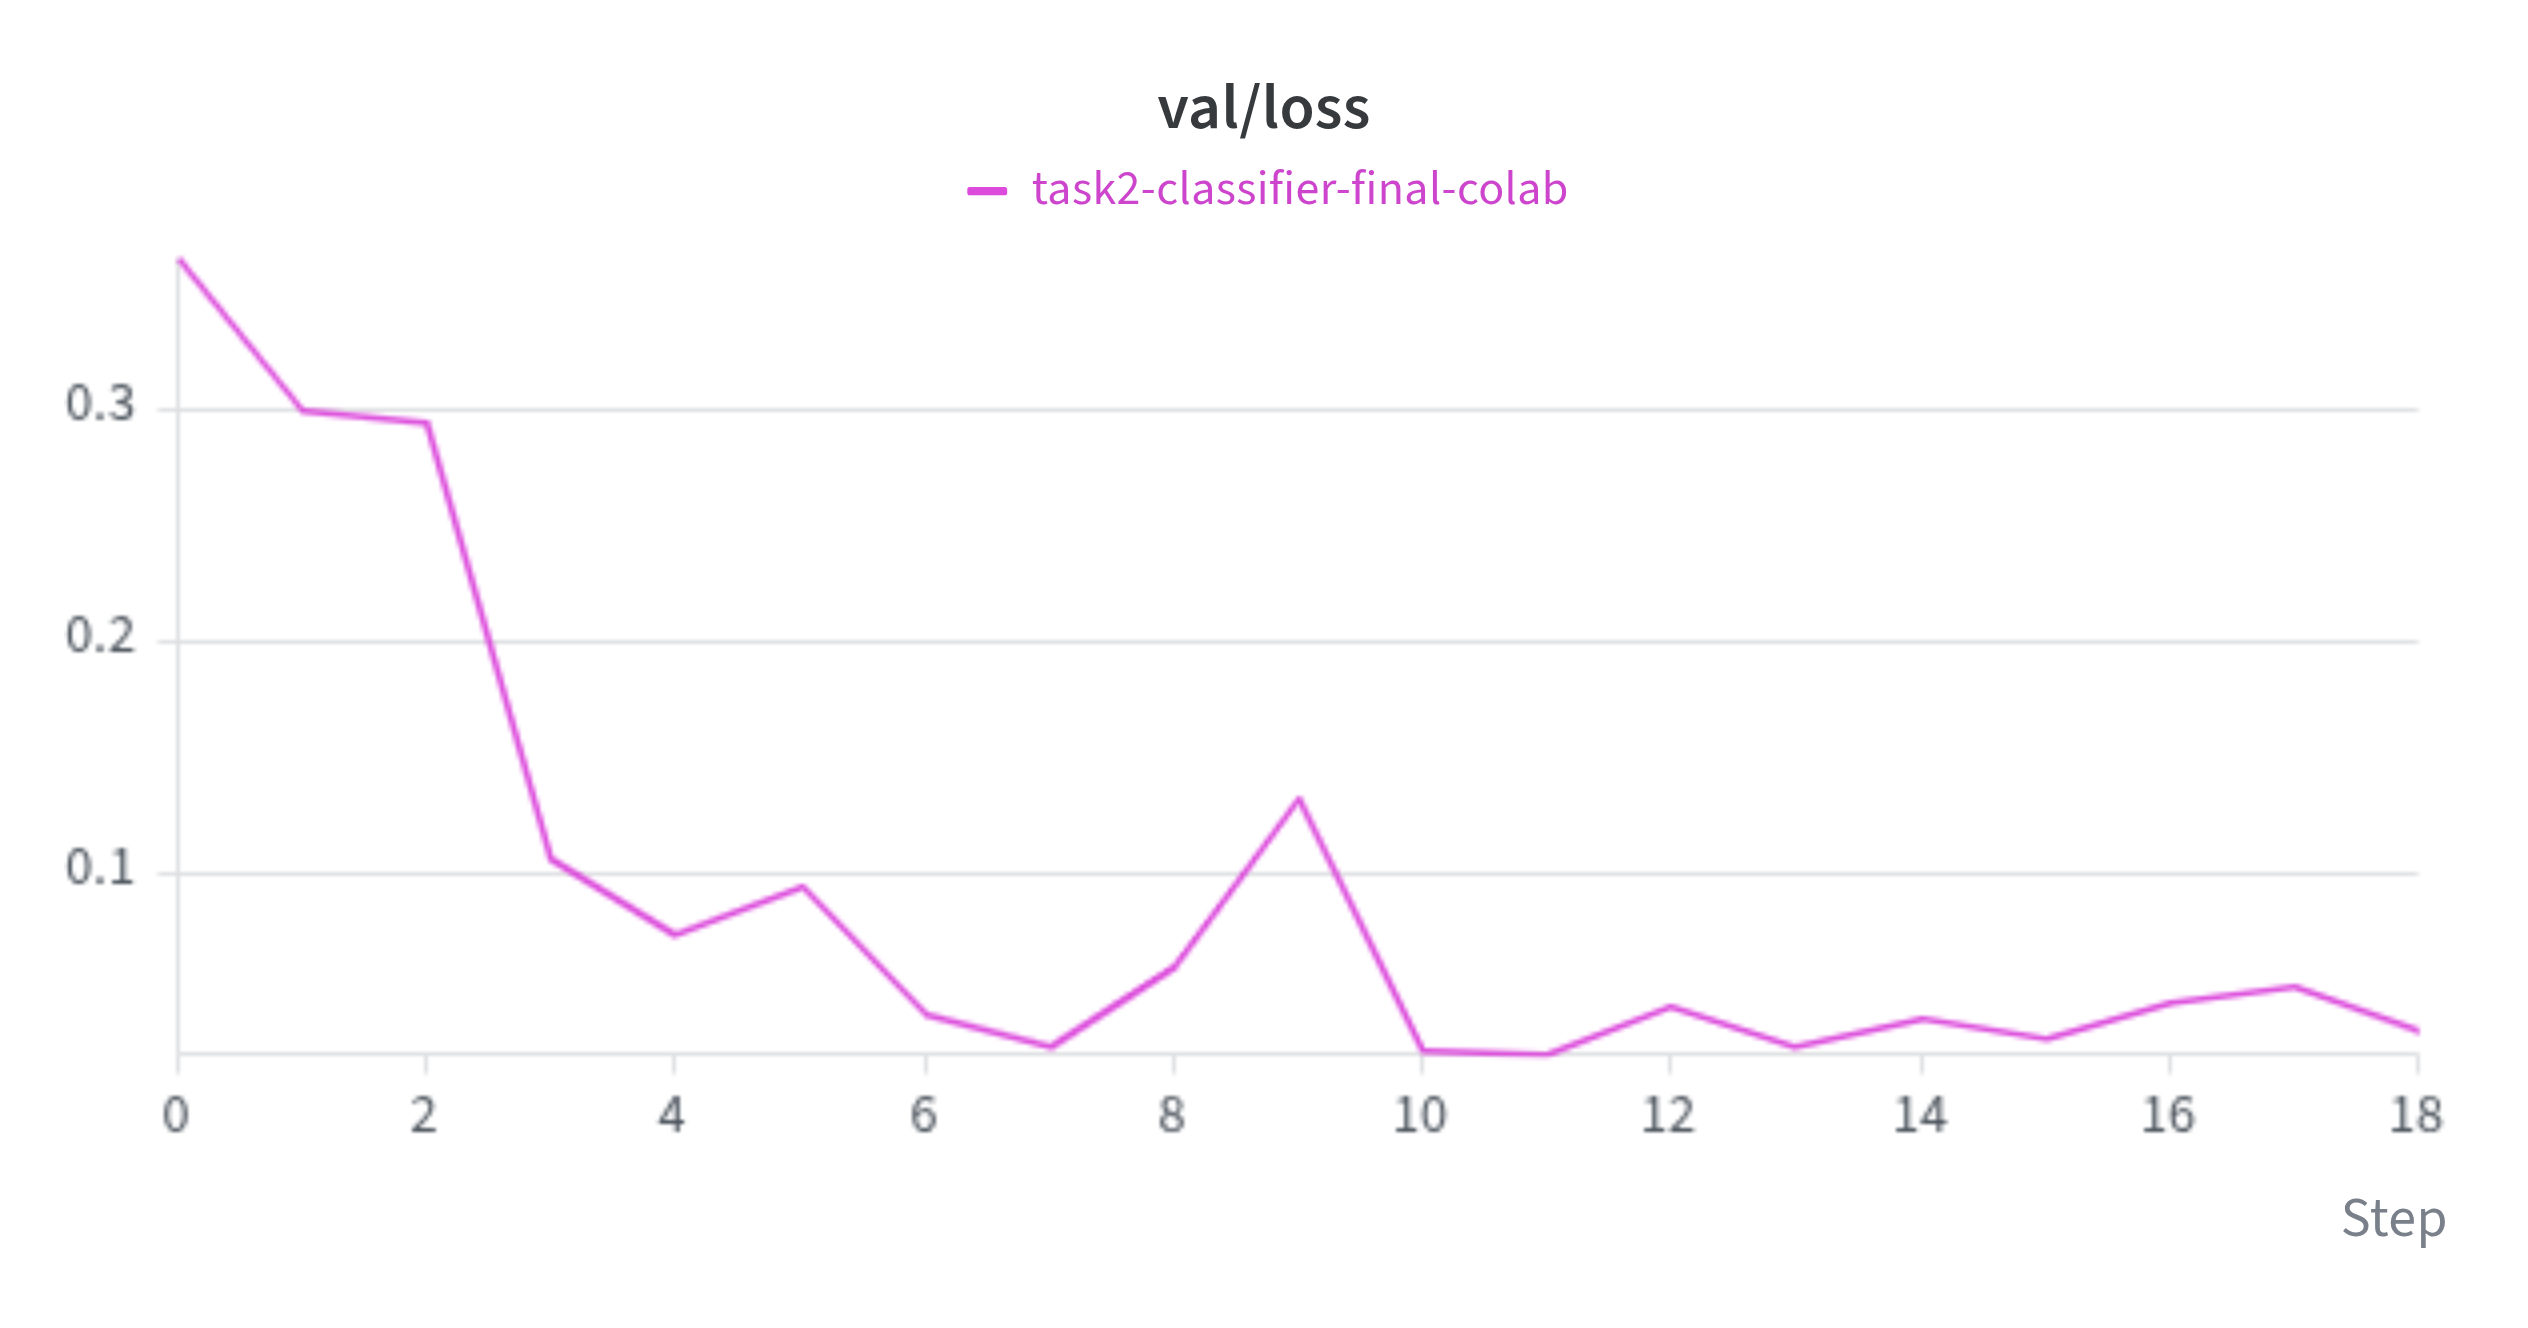
\includegraphics[width=0.24\textwidth]{classifier_val_loss.png}
\caption{Task 2 classifier training traces. Training accuracy rises rapidly and validation accuracy stabilizes near the final high-accuracy regime, while both loss curves decrease with small late fluctuations. The curves support the use of the classifier as an operational router but do not eliminate the need to inspect misrouted examples.}
\label{fig:task2classifiercurves}
\end{figure*}

\begin{figure}[t]
\centering
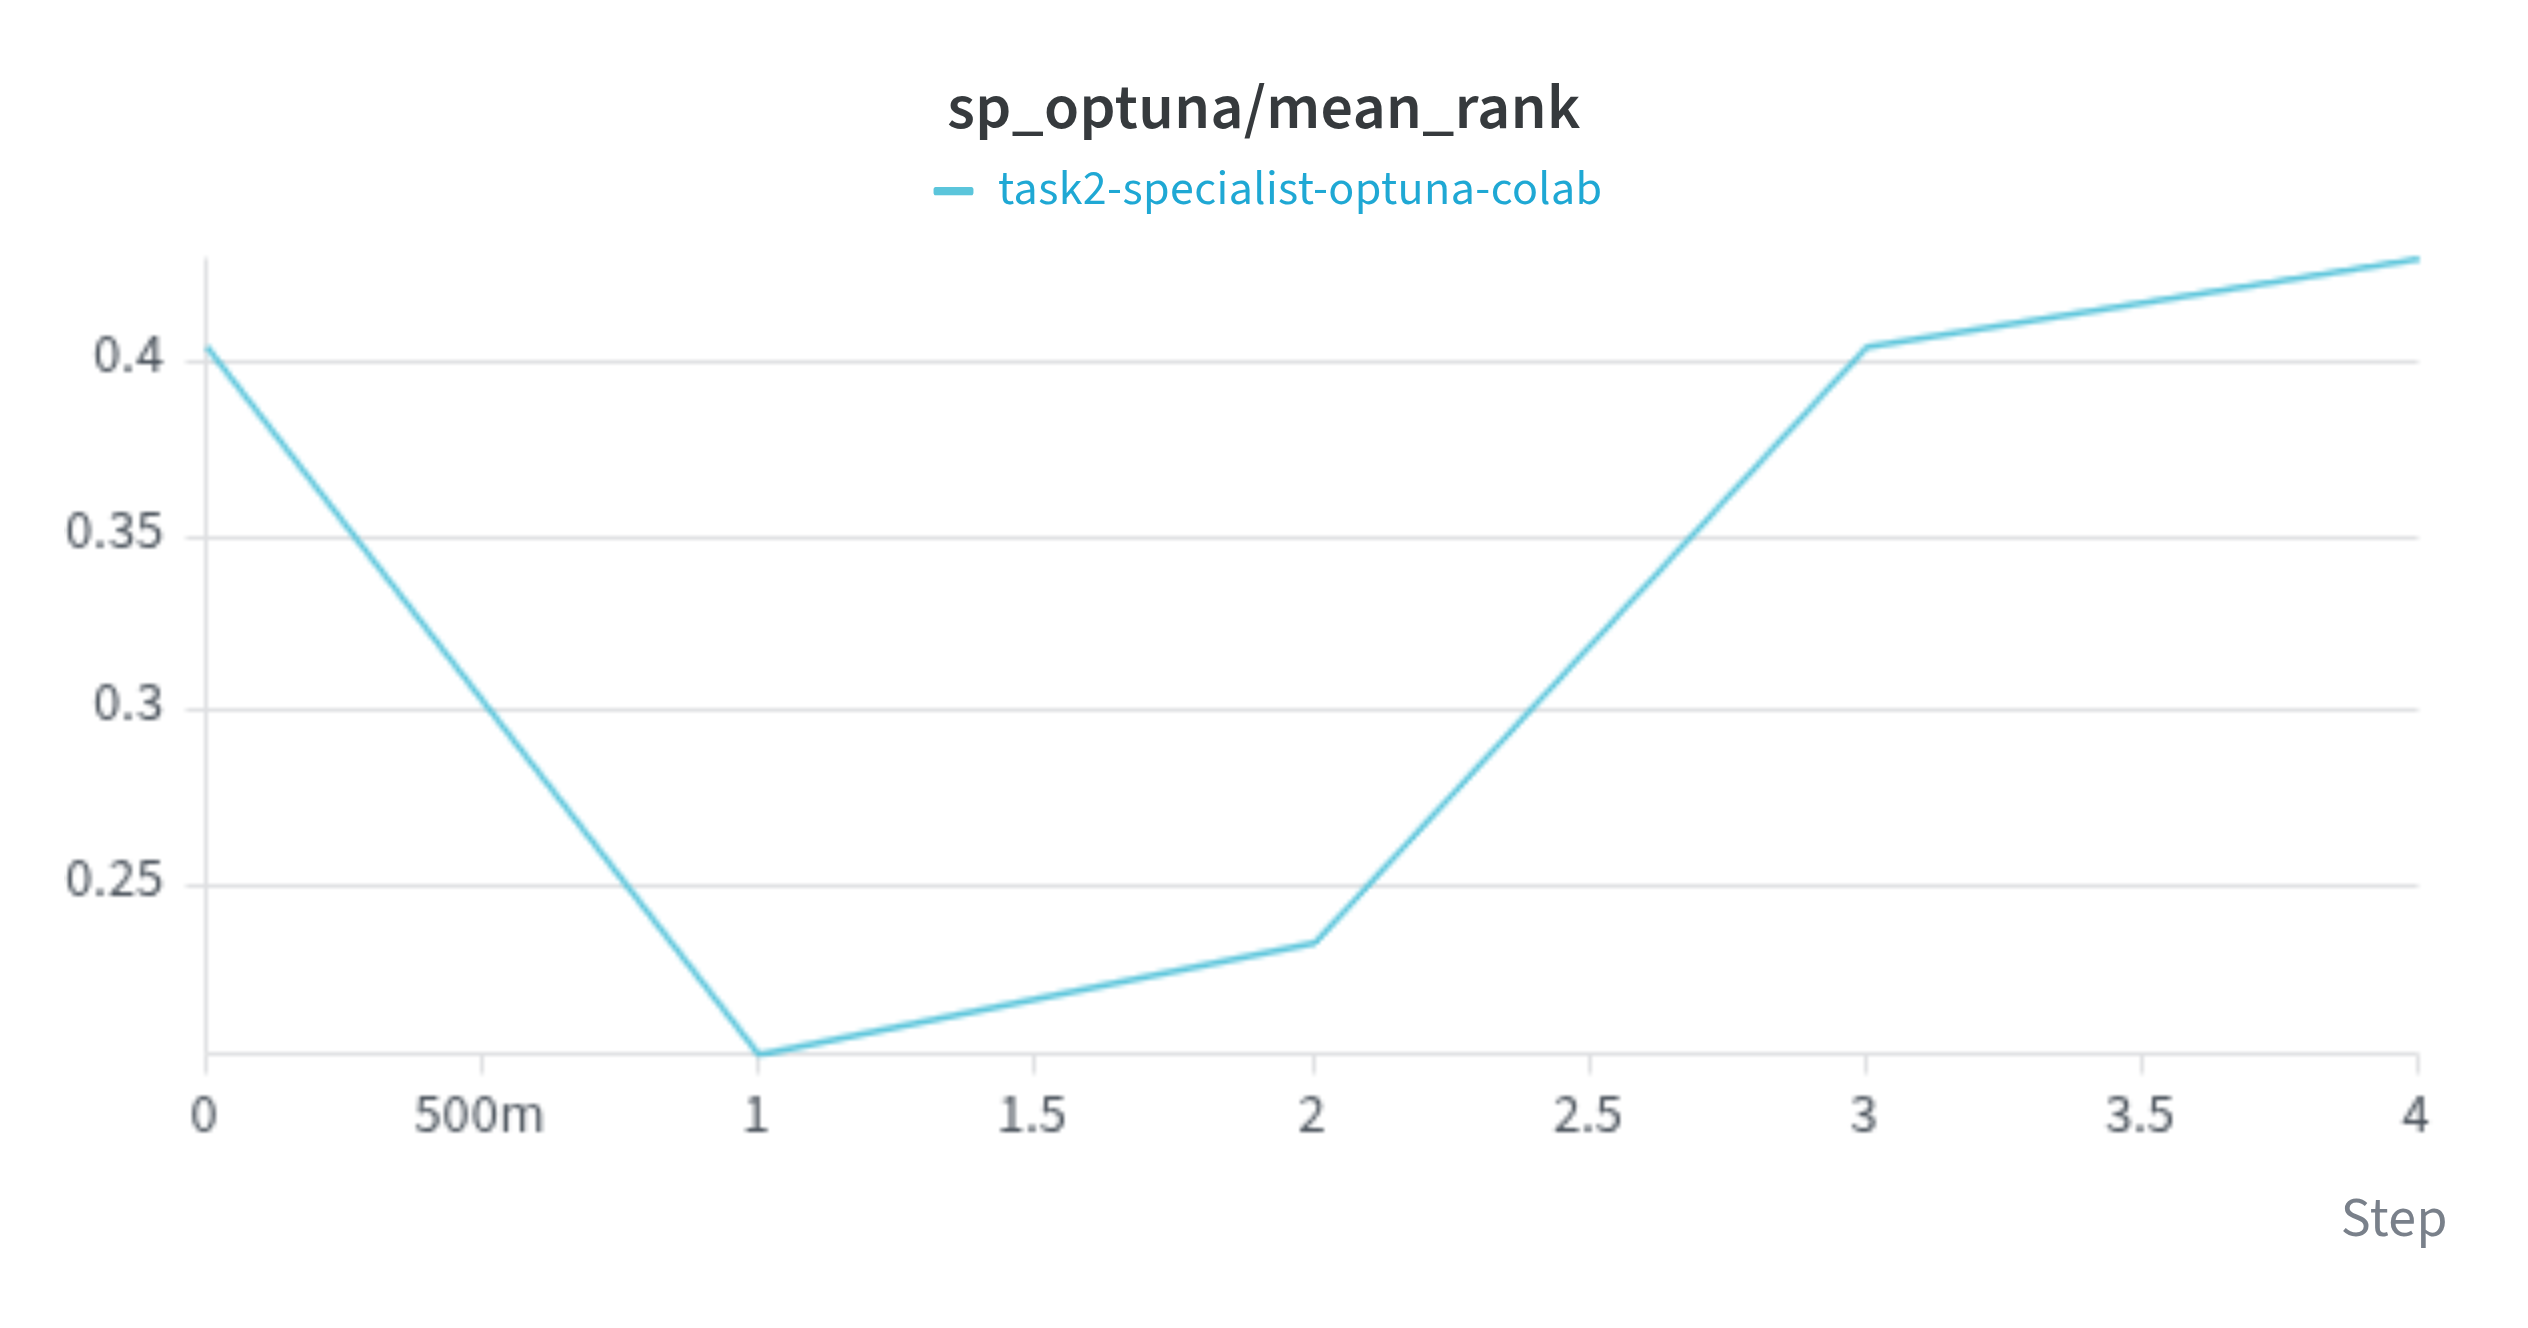
\includegraphics[width=\columnwidth]{sp_oputuna_mean_rank.png}
\caption{Task 2 specialist Optuna mean-ranking objective. Lower is better; the best observed trial is the minimum in the plotted search history.}
\label{fig:task2optuna}
\end{figure}

\section{Task 3: Scope Exclusion}
The assignment specifies a differentiable soft mixture-of-experts model with a gating network, identity branch, specialist initialization from Task 2, warm-up, joint fine-tuning, balance regularization, routing-weight analysis, ONNX export, and a dedicated application workspace. This work did not implement or train Task 3 because the remaining time and available compute were insufficient for a reliable joint training and evaluation cycle. Consequently, no Task 3 architecture, metrics, routing heatmap, ONNX export, or application claim is presented. This is a material gap against the original assignment requirement and is disclosed explicitly rather than represented by unverified results.

\section{Task 4: Conditional Face-to-Sketch GAN}
\subsection{Architecture}
The generator is a seven-stage U-Net encoder with six upsampling stages and skip connections. A learned embedding $e(s)$ represents each of three styles. It is broadcast spatially and concatenated to the photograph before the first generator convolution. The discriminator is a PatchGAN: it concatenates photograph, real/generated sketch, and the broadcast style embedding, then produces a grid of local real/fake logits. This makes the condition visible to both adversarial participants.

\subsection{Objective and training}
The discriminator uses binary cross-entropy with logits on real and fake pairs. The generator minimizes adversarial loss plus paired reconstruction loss:
\begin{equation}
\mathcal{L}_G=\mathcal{L}_{adv}+\lambda_{L1}\|y-G(x,s)\|_1.
\end{equation}
The final configuration recorded in the repository uses 100 epochs, batch size 8, generator learning rate $1.9414\times10^{-4}$, discriminator learning rate $1.4081\times10^{-4}$, 96 base channels, dropout 0.2566, style embedding dimension 4, and $\lambda_{L1}=190.6805$. Optuna searches generator/discriminator learning rates, batch size, base channels, dropout, style dimension, and $\lambda_{L1}$ using a reduced five-epoch trial budget; the selected configuration is then trained for the full schedule. Training logs separate discriminator real/fake losses, generator adversarial/L1 losses, validation L1, and fixed validation image grids through W\&B.

\subsection{Results}
\begin{table}[t]
\caption{Task 4 evaluation results from the supplied metrics artifact.}
\label{tab:task4}
\centering
\begin{tabular}{lccc}
\toprule
Group & L1 & SSIM & $n$\\
\midrule
Overall & 0.22262 & 0.46273 & 1,045\\
Style 1 & 0.16734 & 0.49736 & 618\\
Style 2 & 0.32274 & 0.39268 & 381\\
Style 3 & 0.13611 & 0.57766 & 46\\
\bottomrule
\end{tabular}
\end{table}

Style 3 is strongest on both metrics, while Style 2 is weakest. The unequal group sizes are important: the overall metric is dominated by Styles 1 and 2, so it should not be treated as a uniform estimate of all style categories. L1/SSIM also measure paired similarity rather than the full perceptual quality of a sketch.

\begin{figure}[t]
\centering
\includegraphics[width=0.31\columnwidth]{eval_sample_000_style_2.png}
\includegraphics[width=0.31\columnwidth]{eval_sample_001_style_2.png}
\includegraphics[width=0.31\columnwidth]{eval_sample_002_style_2.png}
\caption{Examples from the supplied Task 4 evaluation output. The fixed evaluation samples provide qualitative evidence alongside the quantitative metrics; style-dependent differences are discussed in the Task 4 analysis.}
\label{fig:task4samples}
\end{figure}

\section{Application Architecture and Deployment}
The backend is a FastAPI service with CORS middleware, upload validation, RGB decoding, bicubic resizing, ONNX Runtime model loading, data-URL image encoding, routing metadata, timing, and metric computation. The frontend is a React/Vite single-page application. The navigation exposes the three completed workspaces and each workspace communicates with its corresponding REST endpoint. Docker Compose starts the backend and frontend containers with one command.

\begin{figure}[t]
\centering
\fbox{\parbox{0.92\columnwidth}{\centering\small
Browser React application\\$\downarrow$\\
FastAPI upload validation and preprocessing\\$\downarrow$\\
ONNX Runtime: Task 1 / Task 2 / Task 4\\$\downarrow$\\
Images, metrics, routing metadata, and downloads}}
\caption{Application architecture. The browser sends an uploaded image and task-specific controls to FastAPI; the selected ONNX graph returns the restored or generated image together with metrics and metadata.}
\label{fig:apparchitecture}
\end{figure}

\begin{figure*}[t]
\centering
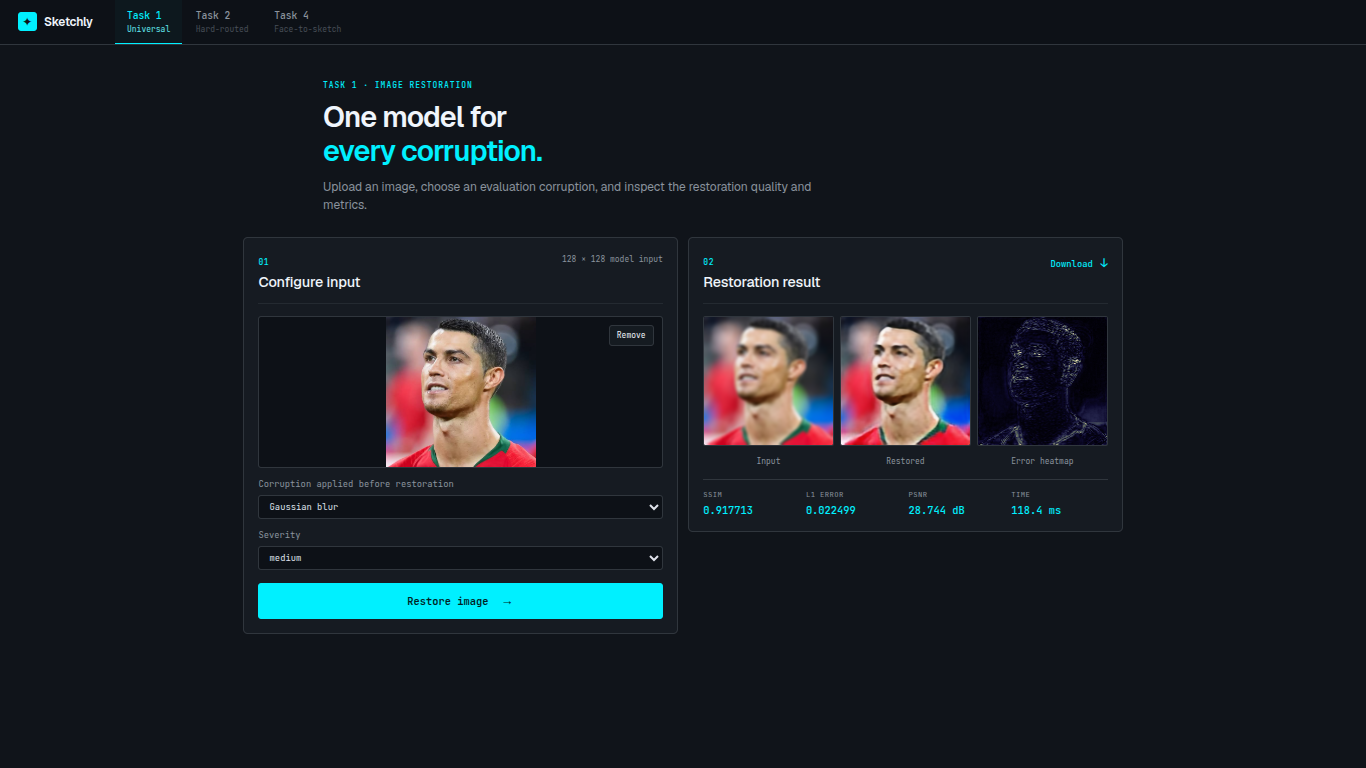
\includegraphics[width=0.32\textwidth]{../screenshots/ui_task1.png}\hfill
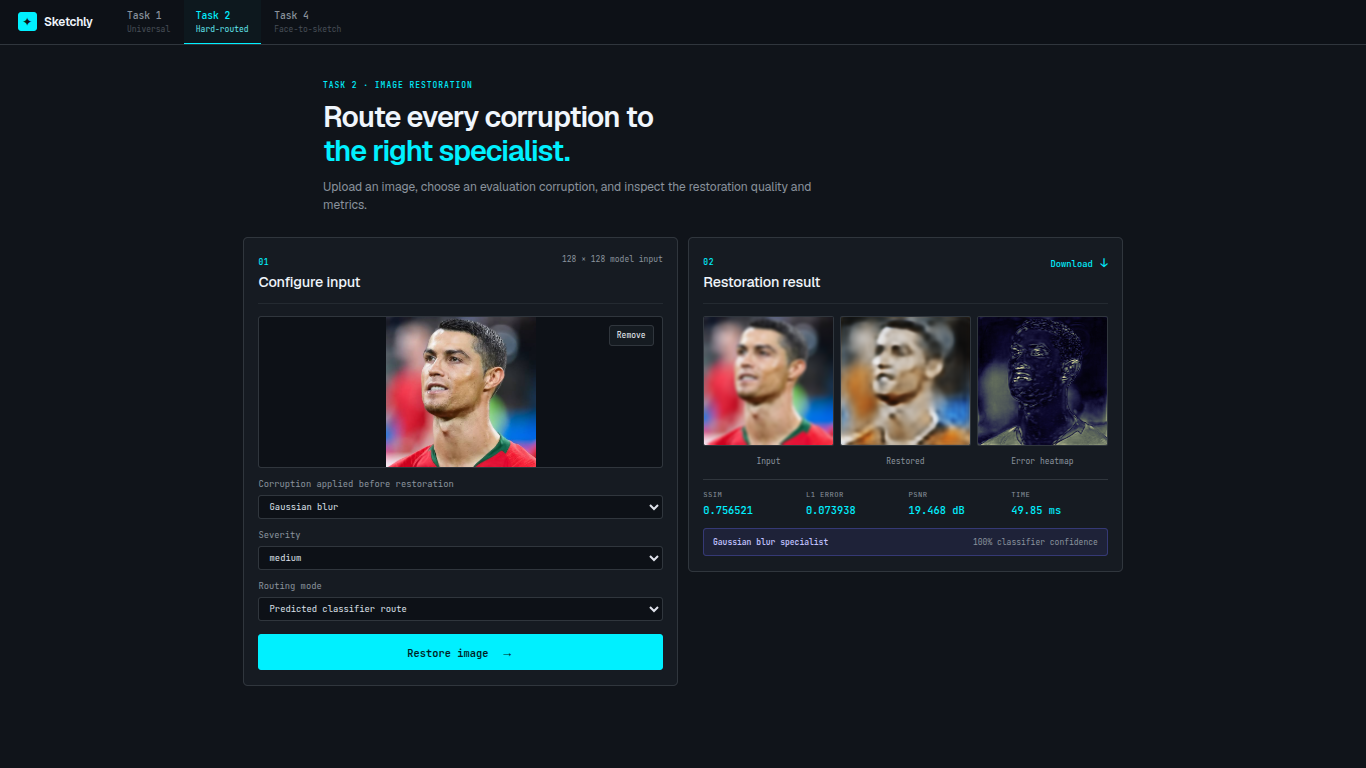
\includegraphics[width=0.32\textwidth]{../screenshots/ui_task2.png}\hfill
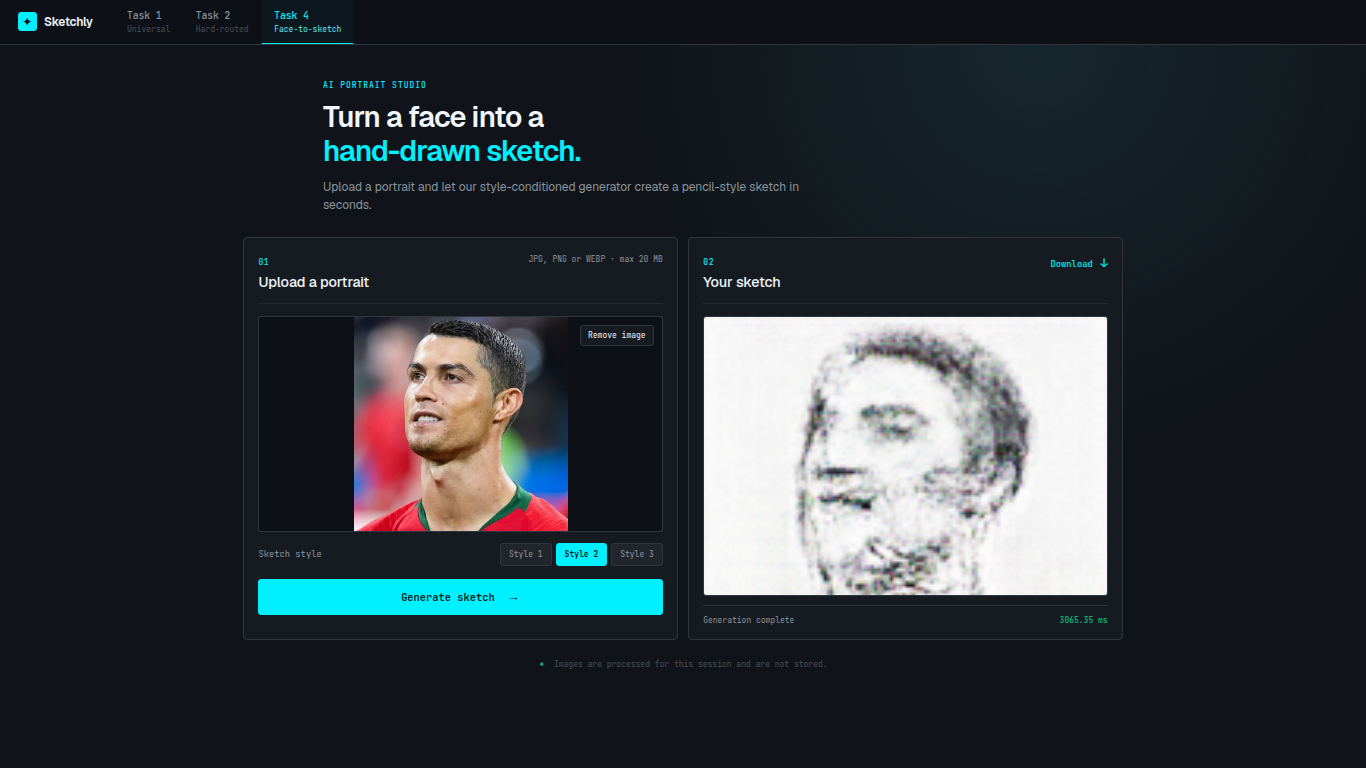
\includegraphics[width=0.32\textwidth]{../screenshots/ui_task4.png}
\caption{Screenshots of the implemented application: (a) universal restoration (Task 1), (b) hard-routed restoration (Task 2), and (c) style-conditioned face-to-sketch generation (Task 4). These captures demonstrate that the three completed pipelines are exposed through a single user interface rather than existing only as offline scripts.}
\label{fig:appscreens}
\end{figure*}

\begin{figure}[t]
\centering
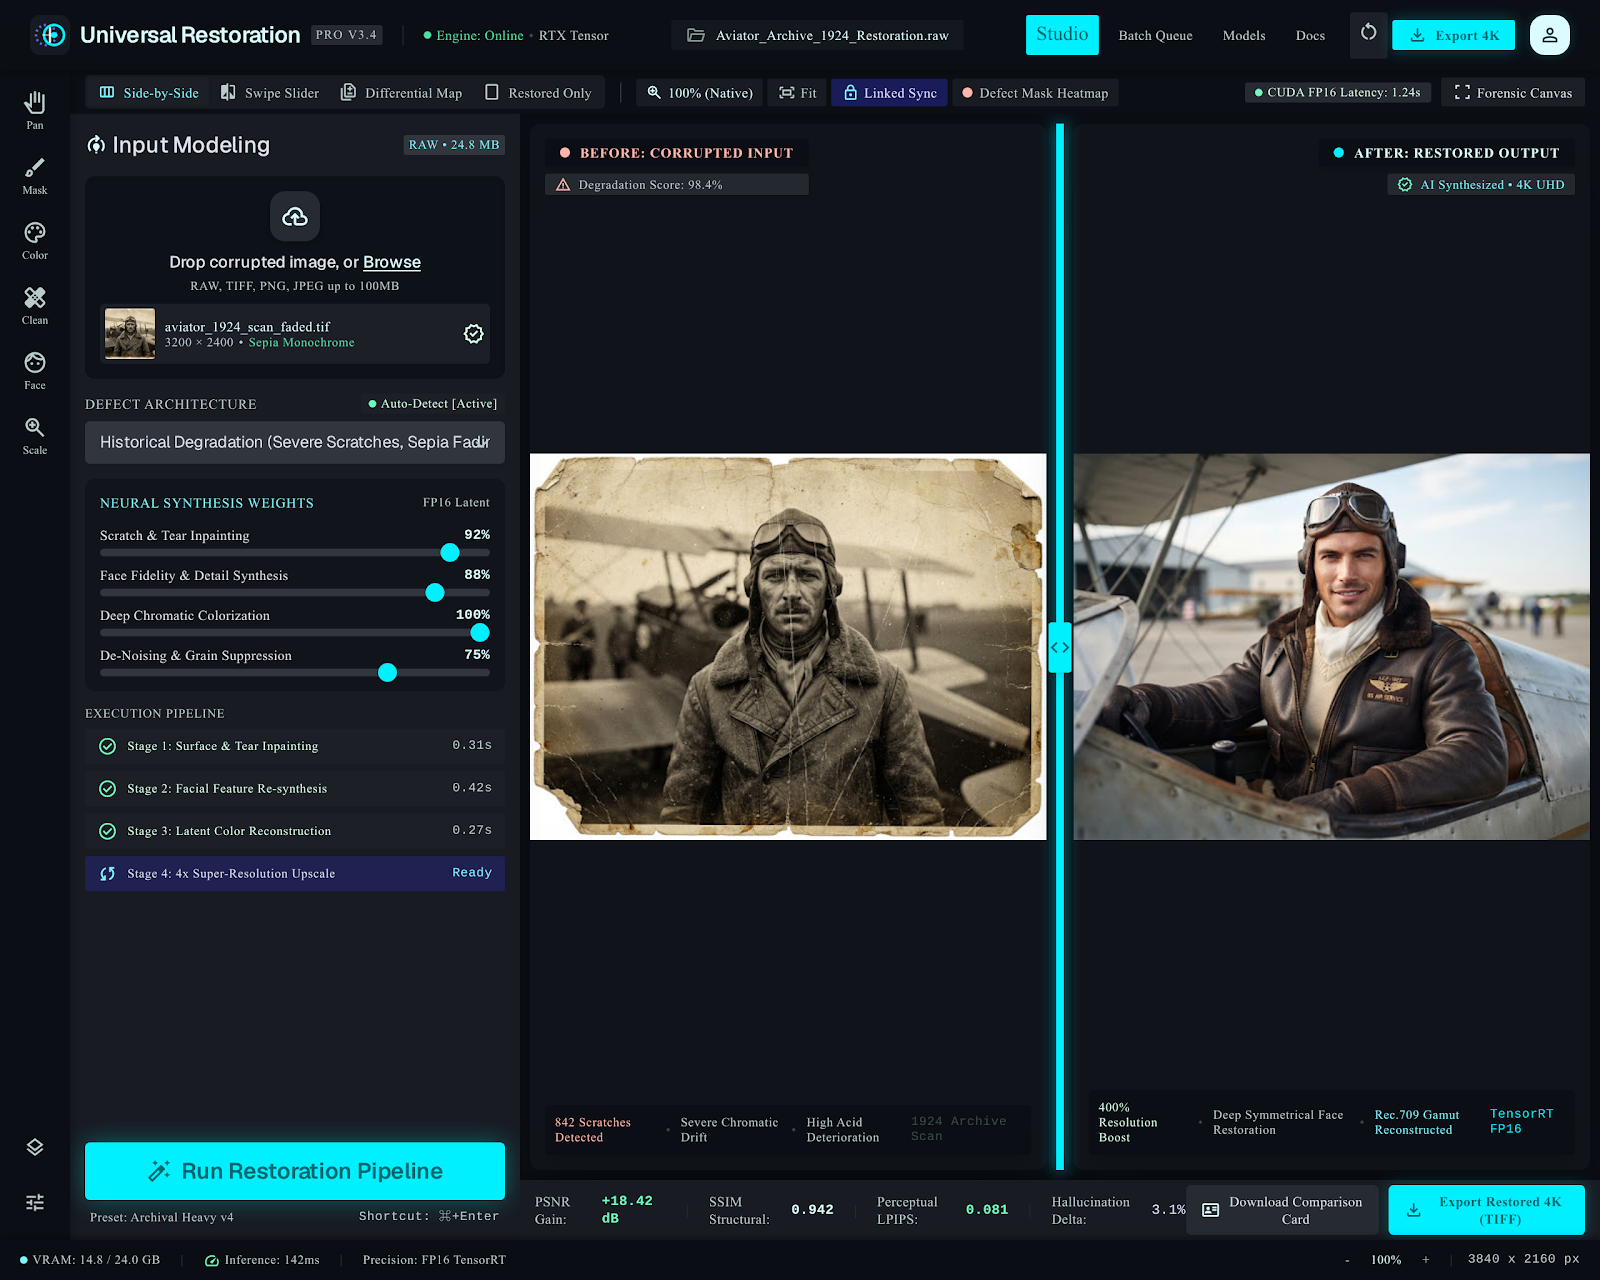
\includegraphics[width=\columnwidth]{../screenshots/google_stitch.png}
\caption{Google Stitch design evidence supplied with the project. The implemented workstation follows the Stitch dark technical palette, cyan interaction state, indigo routing accent, compact technical typography, and dense inspection-panel layout. One Stitch screenshot is included as the available design evidence.}
\label{fig:stitch}
\end{figure}

The model mounts are \texttt{results/task1} to \texttt{/models/task1}, \texttt{results/task2/onnx/onnx} to \texttt{/models/task2}, and \texttt{results/task4/models} to \texttt{/models/task4}. The Task 4 ONNX graph and its external \texttt{.onnx.data} file are mounted together. The application is started with \texttt{docker compose up --build} and opened at \url{http://localhost:5173}.

\section{Verification and Failure Analysis}
ONNX model availability is checked through the backend registry and the application health/metadata endpoints. Interactive smoke tests on previously unseen bundled pet images returned HTTP 200 for both Task 1 and Task 2 after correcting the SSIM implementation. The original failure was a server-side 500 caused by applying one-dimensional `numpy.convolve` directly to a two-dimensional image plane; the fix applies the Gaussian window as separable row and column convolutions.

The most important model-level failure is occlusion restoration, where the target content is absent from the input. The most important routing failure is confusion involving clean images, which are close to low-severity corruptions. For Task 4, Style 2 has the weakest test metrics and should receive focused qualitative inspection. These conclusions are grounded in the supplied metrics and failure grids rather than in a single interactive example.

\section{Experiment Tracking and Submission Evidence}
The repository contains local W\&B CSV exports for Task 1 under \texttt{results/task1/w\&b/skip0.csv}, \texttt{skip1.csv}, and \texttt{skip2.csv}. These exports contain trial configurations, epoch metrics, validation L1/SSIM/ranking values, and final run summaries. The Task 2 directory contains \texttt{best.json}, \texttt{best\_params.json}, \texttt{specialist\_optuna\_results.json}, and \texttt{trials.csv}; these provide the compact search summary and trial-level records even though separate W\&B CSV exports for Task 2 are not present locally. Figures~\ref{fig:task1curves}, \ref{fig:task2classifiercurves}, and \ref{fig:task2optuna} use the graph files added to the repository. No local Task 4 W\&B run directory or synchronized Task 4 curve export was found, so Task 4 is represented by its verified quantitative metrics and fixed evaluation sample grid rather than reconstructed training curves.

The Google Stitch evidence is included in Fig.~\ref{fig:stitch}, and the implemented workspaces are shown in Fig.~\ref{fig:appscreens}. The GitHub repository is \url{https://github.com/AKIF-jk/Generative_AI}. A demonstration of the application is available at \url{https://youtu.be/XWOXw59H3mw}.

\section{Limitations}
The current repository does not contain a completed Task 3 implementation. Synchronized Task 4 W\&B training curves are unavailable because the original runs were stored locally and were not synced; the report therefore uses the verified quantitative metrics and fixed evaluation grid for Task 4. Task 1's local CSV exports were treated as supporting experiment records because W\&B exports may contain repeated epoch rows from multiple runs. These limitations are reported to keep the manuscript auditable.

\section{Conclusion}
The completed system demonstrates a full path from deterministic data preparation and model evaluation to ONNX inference and browser deployment for Tasks 1, 2, and 4. The universal restoration model provides a strong shared baseline, while Task 2 exposes the value and risks of explicit corruption routing. The conditional GAN demonstrates style-dependent paired generation, with performance varying substantially by style. The application makes these behaviours inspectable through a single Dockerized interface. The exclusion of Task 3 remains the principal limitation relative to the original four-task specification.

\section*{AI Use and Verification Appendix}
AI-assisted tools were used for code navigation, frontend implementation, debugging, and report drafting. Generated suggestions were checked against the assignment PDF, the repository source, result JSON files, Docker Compose behaviour, production frontend builds, Python compilation, and live HTTP smoke tests. The SSIM issue reported in this work was diagnosed from backend logs and corrected in the source rather than hidden behind a frontend error message.

\begin{thebibliography}{00}
\bibitem{wang2004ssim} Z. Wang, A. C. Bovik, H. R. Sheikh, and E. P. Simoncelli, ``Image quality assessment: From error visibility to structural similarity,'' \emph{IEEE Trans. Image Process.}, vol. 13, no. 4, pp. 600--612, 2004.
\bibitem{isola2017pix2pix} P. Isola, J.-Y. Zhu, T. Zhou, and A. A. Efros, ``Image-to-image translation with conditional adversarial networks,'' in \emph{Proc. IEEE CVPR}, 2017, pp. 1125--1134.
\bibitem{fan2022fs2k} D.-P. Fan, Z. Huang, P. Zheng, H. Liu, X. Qin, and L. Van Gool, ``Facial-sketch synthesis: A new challenge,'' \emph{Machine Intelligence Research}, vol. 19, pp. 257--287, 2022.
\bibitem{goodfellow2014gan} I. Goodfellow et al., ``Generative adversarial nets,'' in \emph{Advances in Neural Information Processing Systems}, 2014.
\bibitem{bergstra2012random} J. Bergstra and Y. Bengio, ``Random search for hyper-parameter optimization,'' \emph{J. Mach. Learn. Res.}, vol. 13, pp. 281--305, 2012.
\bibitem{akiba2019optuna} T. Akiba, S. Sano, T. Yanase, T. Ohta, and M. Koyama, ``Optuna: A next-generation hyperparameter optimization framework,'' in \emph{Proc. ACM KDD}, 2019, pp. 2623--2631.
\bibitem{heusel2017fid} M. Heusel, H. Ramsauer, T. Unterthiner, B. Nessler, and S. Hochreiter, ``GANs trained by a two time-scale update rule converge to a local Nash equilibrium,'' in \emph{Advances in Neural Information Processing Systems}, 2017.
\bibitem{zhang2018lpips} R. Zhang, P. Isola, A. A. Efros, E. Shechtman, and O. Wang, ``The unreasonable effectiveness of deep features as a perceptual metric,'' in \emph{Proc. IEEE CVPR}, 2018, pp. 586--595.
\end{thebibliography}

\end{document}
